\section{Results}
The SaltProc online reprocessing simulation package is demonstrated in four 
applications: (1) analyzing  \gls{MSBR} neutronics and fuel cycle to find the 
equilibrium core composition and core depletion, (2) studying operational and 
safety parameters evolution during \gls{MSBR} operation, (3) demonstrating that 
in a single-fluid two-region \gls{MSBR} conceptual design the undermoderated 
outer core zone II works as a virtual ``blanket", reduces neutron leakage and 
improves breeding ratio due to neutron energy spectral shift, and (4) 
determining the effect of fission product removal on the core neutronics.

The neutron population per cycle and the number of active/inactive cycles were 
chosen to obtain balance between reasonable uncertainty for a transport problem 
($\leq$ 15 pcm\footnote{ 1 pcm = 10$^{-5}\Delta k_{eff}/k_{eff}$} for effective 
multiplication factor) and computational time. The \gls{MSBR} depletion and 
safety parameter computations were performed on 64 Blue Waters XK7 nodes (two 
AMD 6276 Interlagos CPU per node, 16 floating-point Bulldozer core units per 
node or 32 ``integer" cores per node, nominal clock speed is 2.45 GHz). The 
total computational time for calculating the equilibrium composition was 
approximately 9,900 node-hours (18 core-years.)

\subsection{Effective multiplication factor}
Figure~\ref{fig:keff} shows the effective multiplication factors 
obtained using SaltProc and SERPENT 2. The effective multiplication factors were 
calculated after removing fission products listed in 
Table~\ref{tab:reprocessing_list} and adding the fertile material at the end of 
cycle time (3 days for this work). The effective multiplication 
factor fluctuates significantly as a result of the batch-wise nature of this 
online reprocessing strategy. 

\begin{figure}[ht!] 
  \centering
  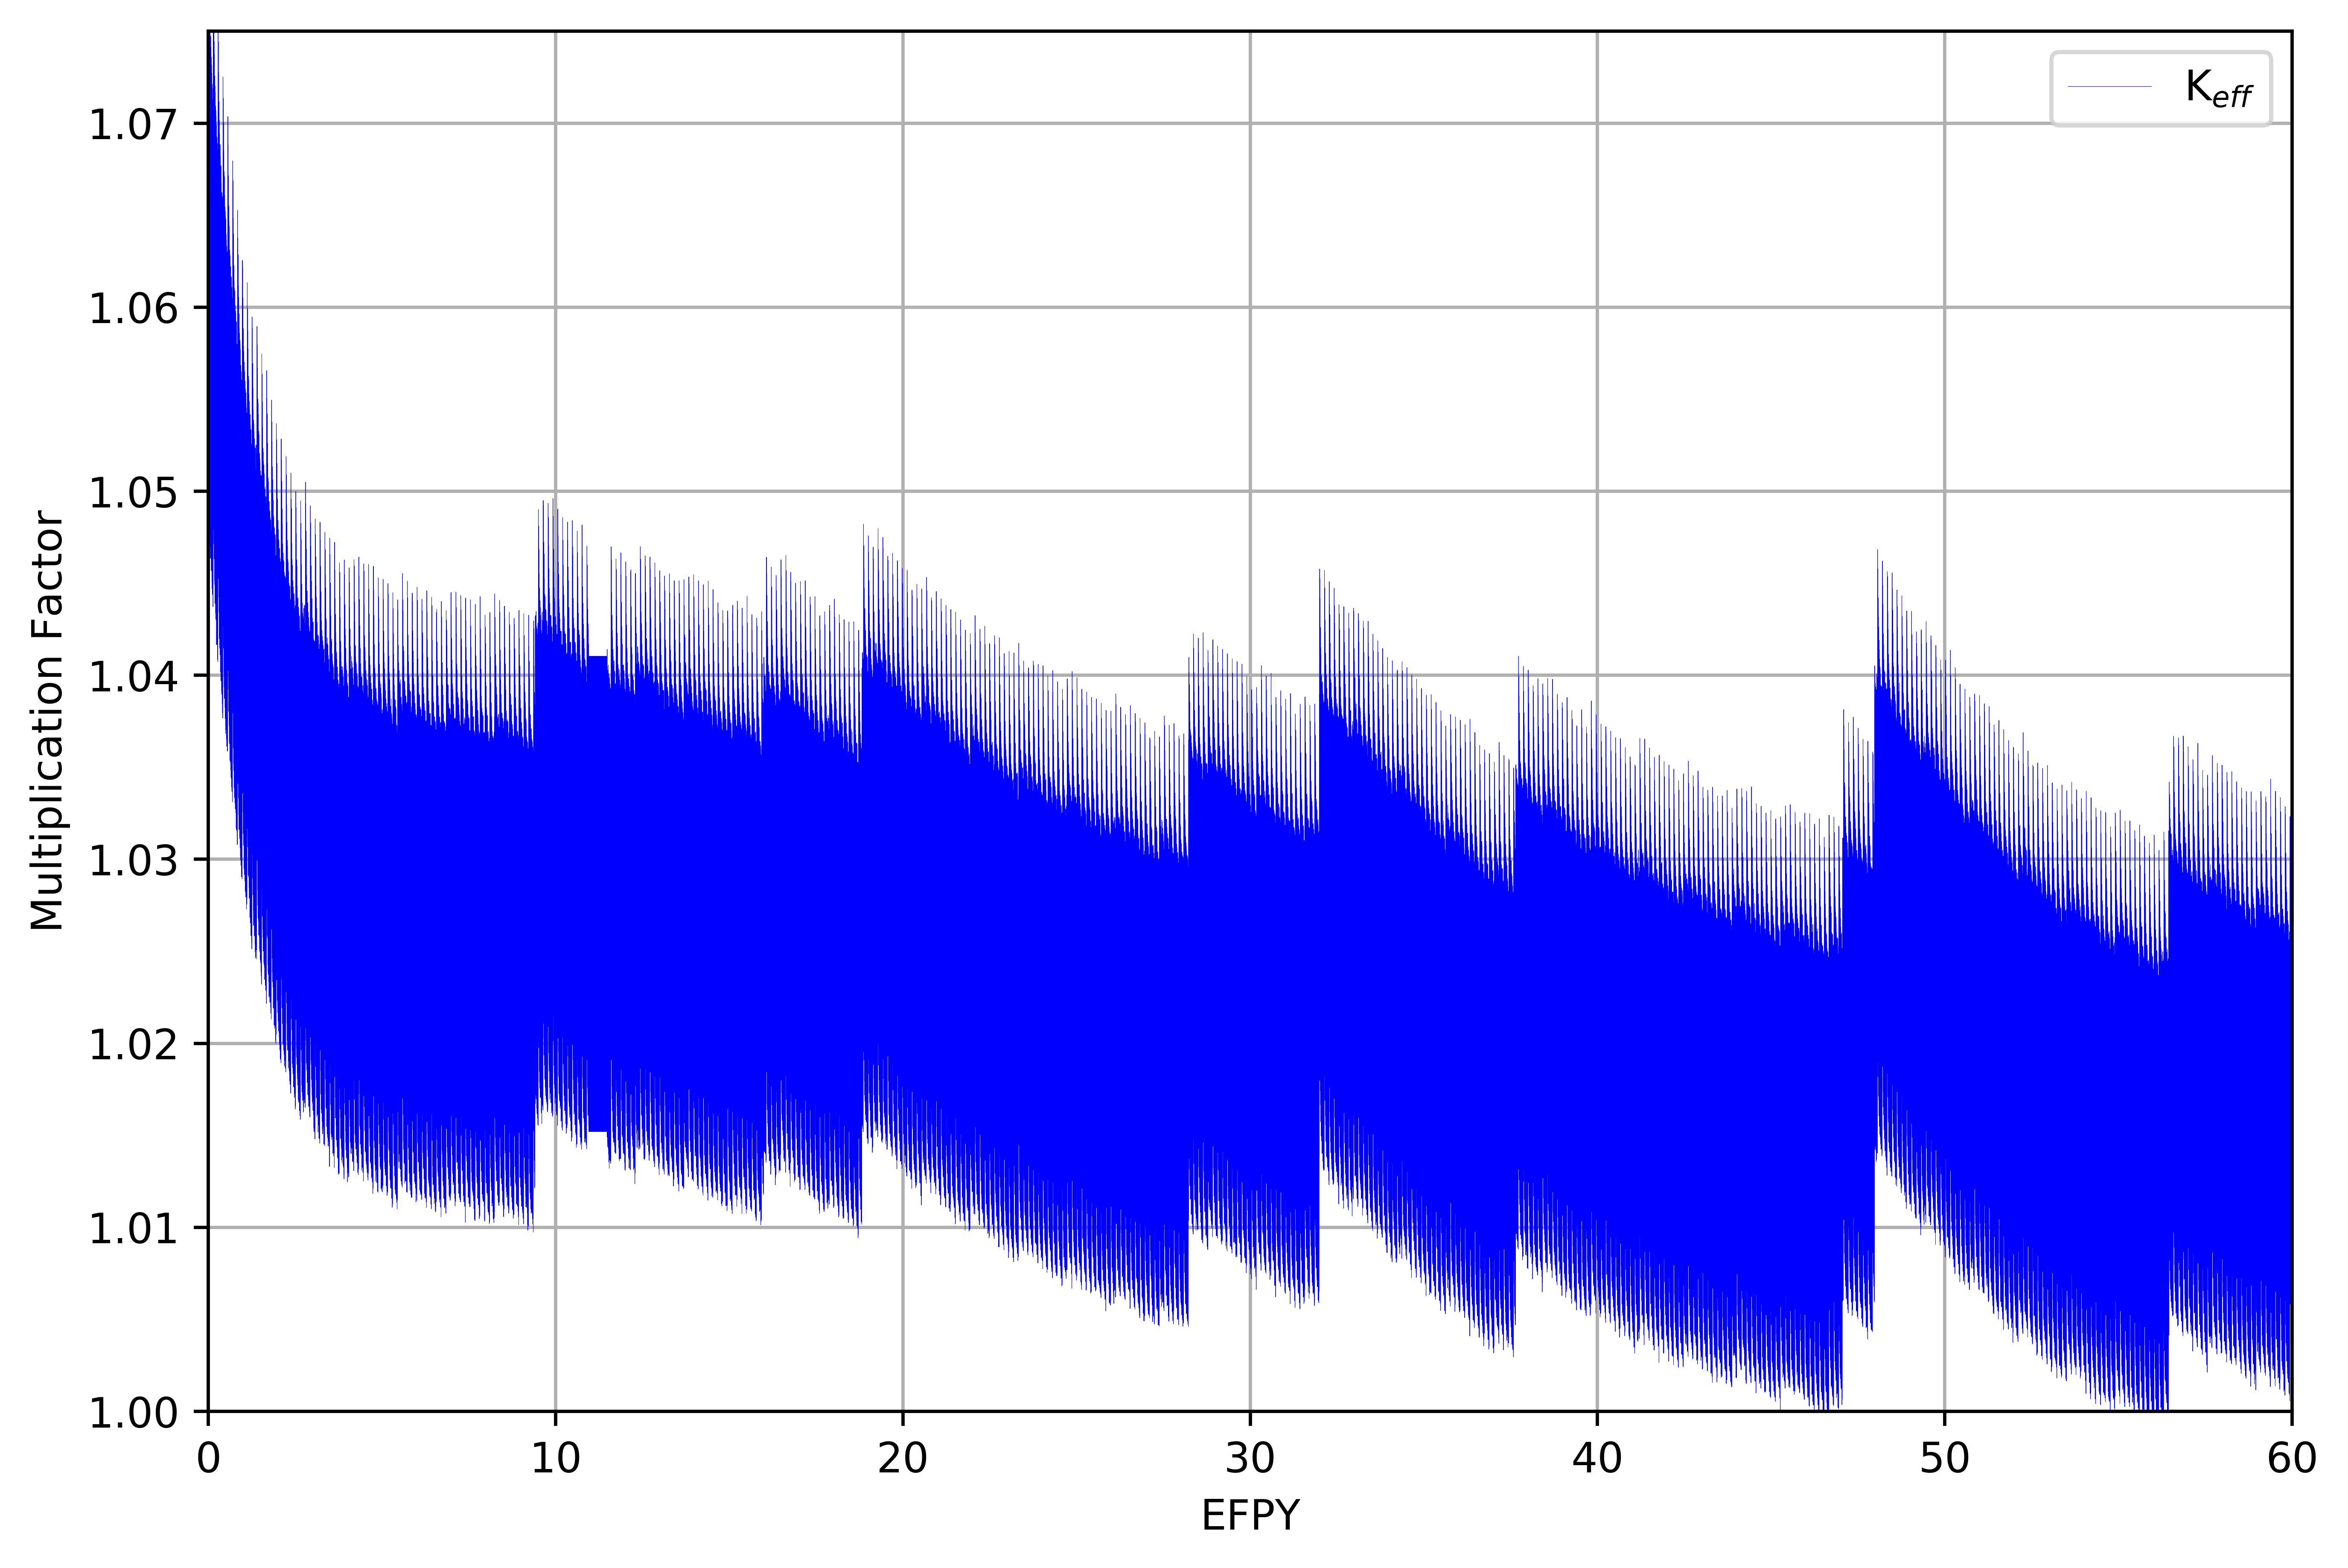
\includegraphics[width=\textwidth]{keff.png}
  \caption{Effective multiplication factor dynamics for full-core \gls{MSBR} 
  model over a 60-year reactor operation lifetime.}
  \label{fig:keff}
\end{figure}

First, SERPENT calculates the effective multiplication factor for the beginning 
of the cycle (there is fresh fuel composition at the first step). Next, it 
computes the new fuel salt composition at the end of a 3-day depletion. The 
corresponding effective multiplication factor is much smaller than the previous 
one. Finally, SERPENT calculates $k_{eff}$ for the depleted composition after 
applying feeds and removals. The $K_{eff}$ increases accordingly since major reactor 
poisons (e.g. Xe, Kr) are removed, while fresh fissile material ($^{233}$U) 
from the protactinium decay tank is added.  

Additionally, the presence of rubidium, strontium, cesium, and barium in the 
core are disadvantageous to reactor physics. In fact, SaltProc fully removes all these elements every 3435 days (not a small mass fraction every 3 days) 
which causes the multiplication factor to jump by approximately 450 
pcm, and limits using the batch approach for online reprocessing simulations. 
In future versions of SaltProc this drawback will be eliminated by removing 
elements with longer residence times (seminoble metals, volatile fluorides, Rb, Sr,
 Cs, Ba, Eu) using different approach. Only mass fraction (calculated 
 separately for each reprocessing group) will be removed every depletion step 
 (e.g. 3 days) instead of removing 100\% of element atoms after cycle time.
Overall, the effective multiplication factor gradually decreases from 1.075 to 
$\approx$1.02 at equilibrium after approximately 6 years of irradiation. 

\subsection{Fuel salt composition dynamics}
The analysis of the fuel salt composition evolution provides more comprehensive 
information about the equilibrium state. Figure~\ref{fig:adens_eq} shows the number 
densities of major nuclides which have a strong influence on the reactor core 
physics. The concentration of $^{233}$U, $^{232}$Th, $^{233}$Pa, and $^{232}$Pa in 
the fuel salt change insignificantly after approximately 2500 days of operation. 
In particular, the $^{233}$U number density fluctuates by less than 0.8\% between
 16 and 20 years of operation. Hence, a quasi-equilibrium state was 
achieved after 16 years of reactor operation.
\begin{figure}[ht!] % replace 't' with 'b' to 
  \centering
  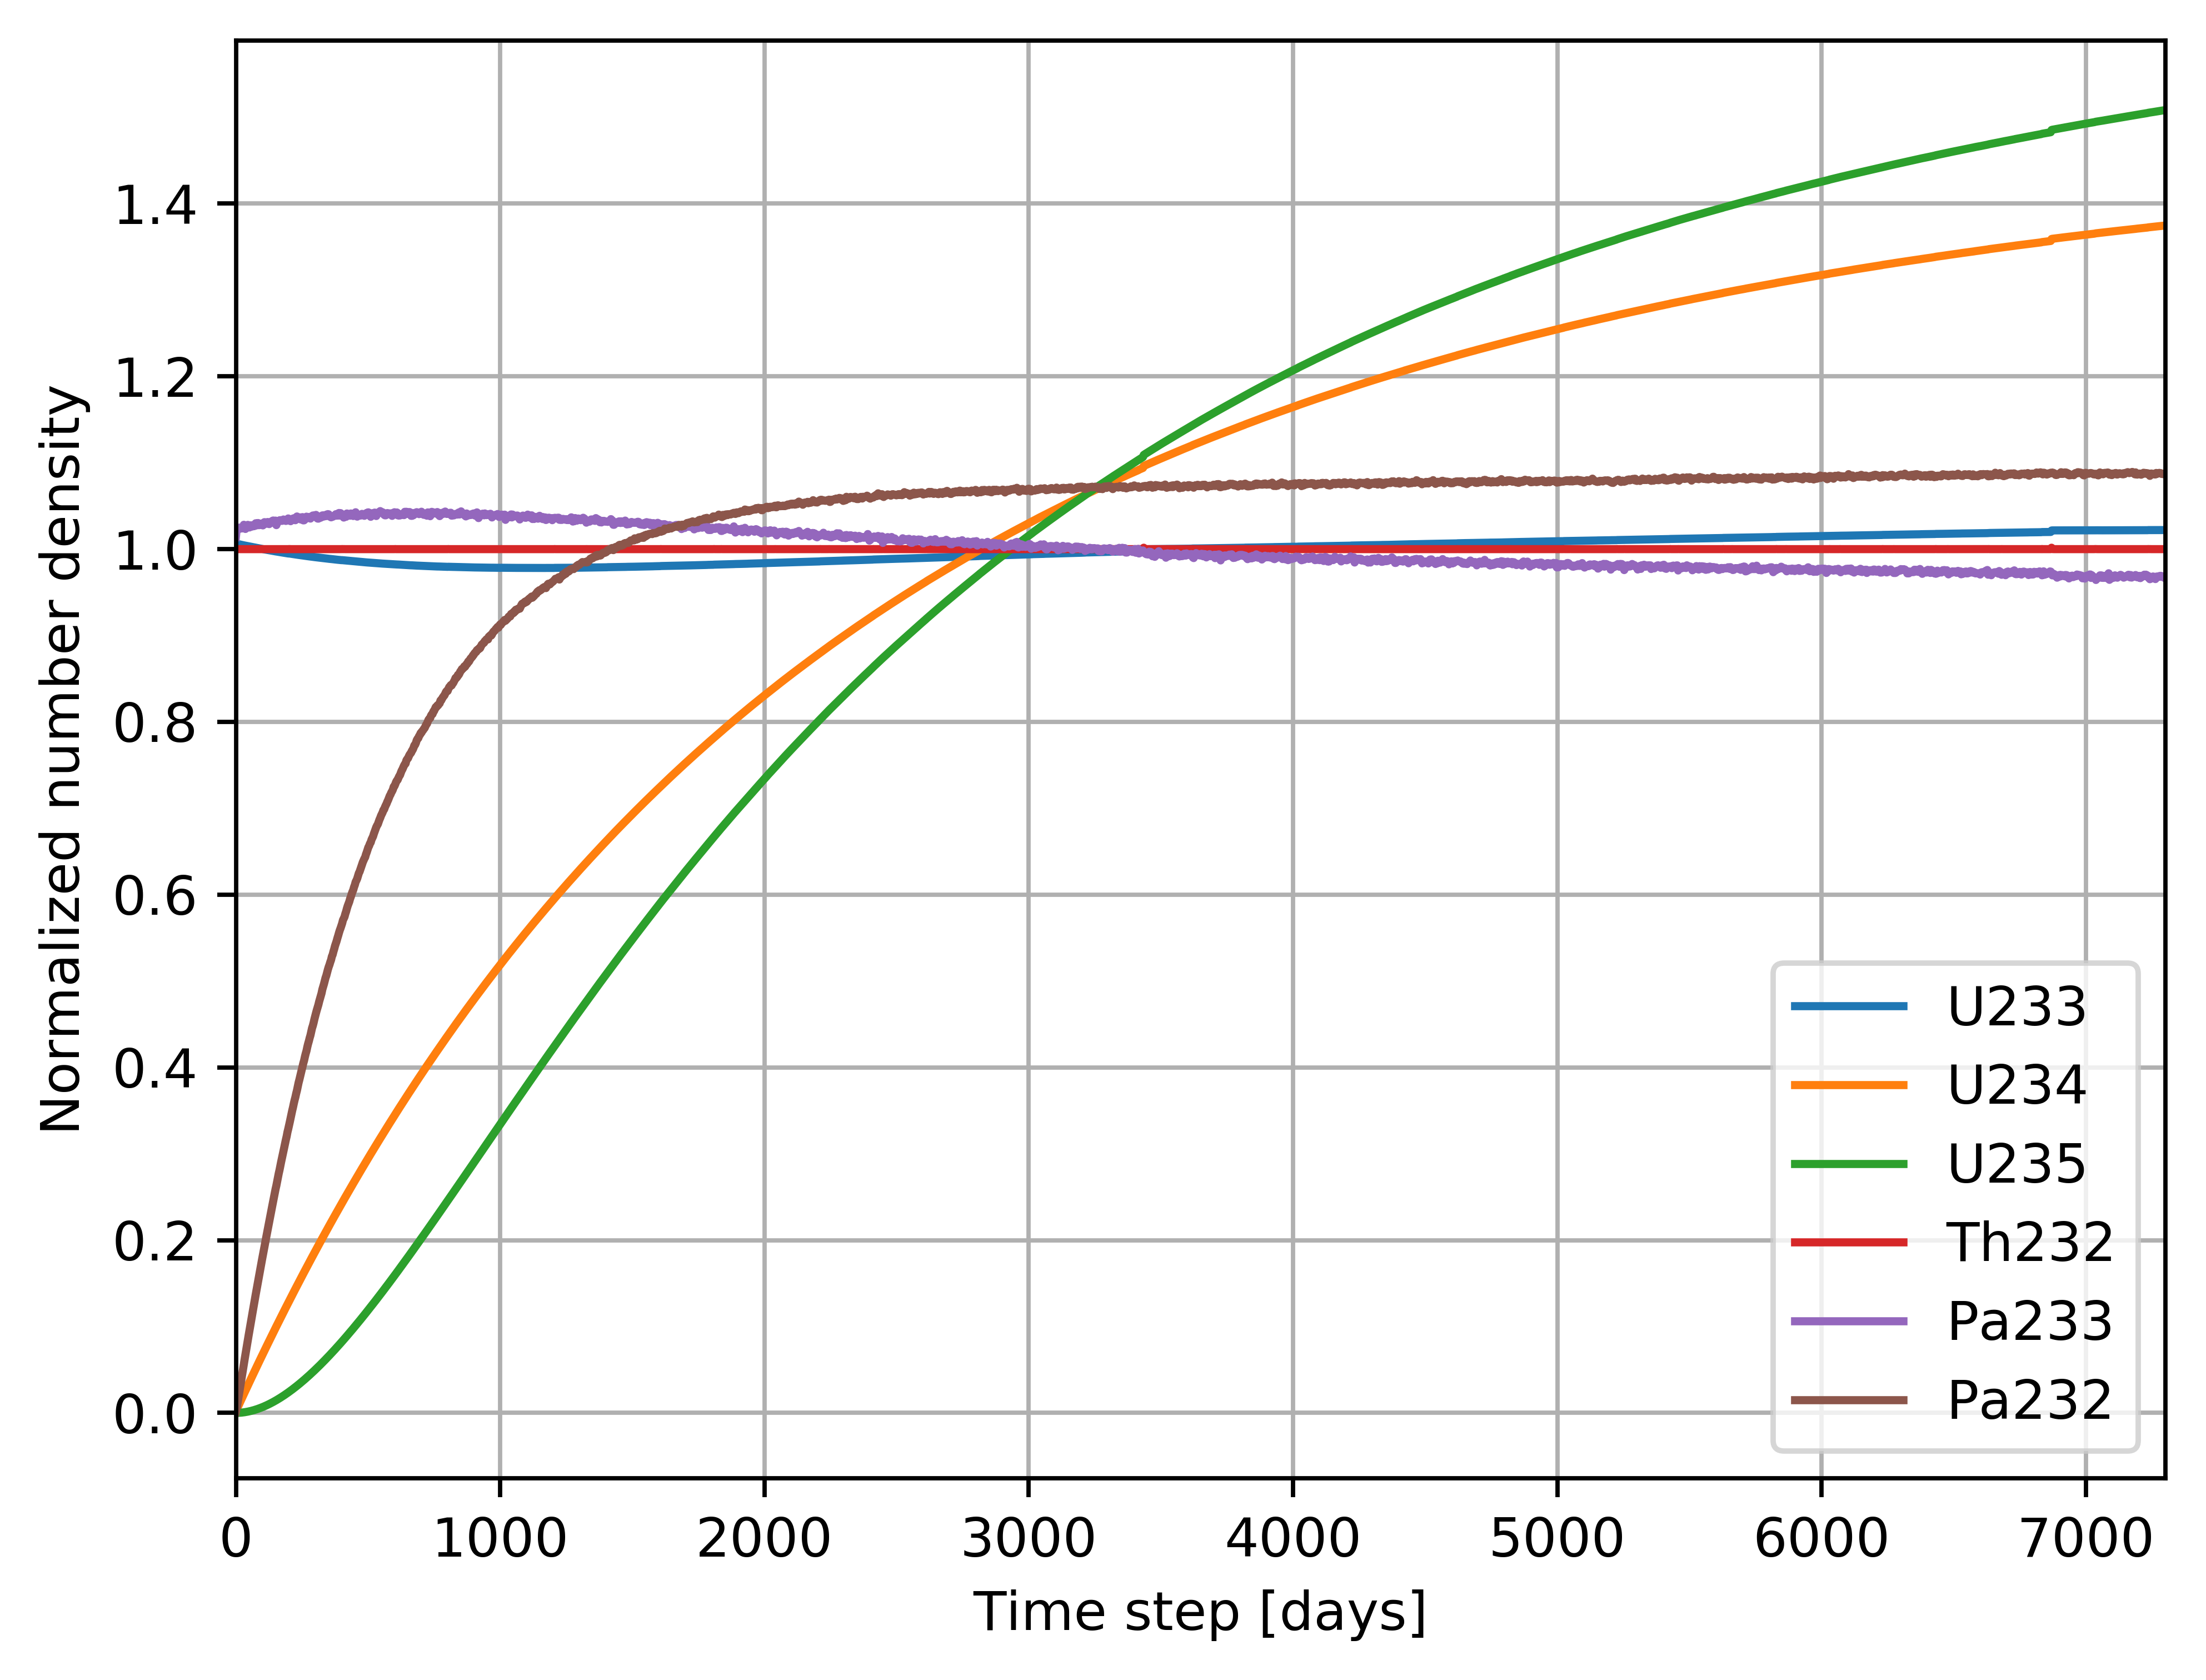
\includegraphics[width=\textwidth]{major_isotopes_adens.png}
  \caption{Number density of major nuclides during 60 years of reactor 
  operation.}
  \label{fig:adens_eq}
\end{figure}
In contrast, a wide variety of nuclides, including fissile isotopes (e.g. 
$^{235}$U) and non-fissile strong absorbers (e.g. $^{234}$U), kept accumulating 
in the core. Figure~\ref{fig:fissile_short} demonstrates production of fissile 
isotopes in the core. In the end of the considered operational time, the core 
contained significant $^{235}$U ($\approx10^{-5}$ atom/b-cm), $^{239}$Pu 
($\approx5\times10^{-7}$ atom/b-cm), and $^{241}$Pu ($\approx 5\times10^{-7}$ 
atom/b-cm). Meanwhile, the equilibrium number density of the target fissile 
isotope $^{233}$U was approximately 7.97$\times10^{-5}$ atom/b-cm. Small dips 
in neptunium and plutonium number density every 16 years are caused by removing
$^{237}$Np, $^{242}$Pu (included in Processing group ``Higher nuclides'', see
 Table~\ref{tab:reprocessing_list}) which decays into $^{235}$Np, $^{239}$Pu, 
 respectively. Thus, 
production of new fissile materials in the core, as well as $^{233}$U breeding, 
made it possible to compensate for negative effects of strong absorber 
accumulation and keep the reactor critical.
\begin{figure}[htp!] % replace 't' with 'b' to 
  \centering
  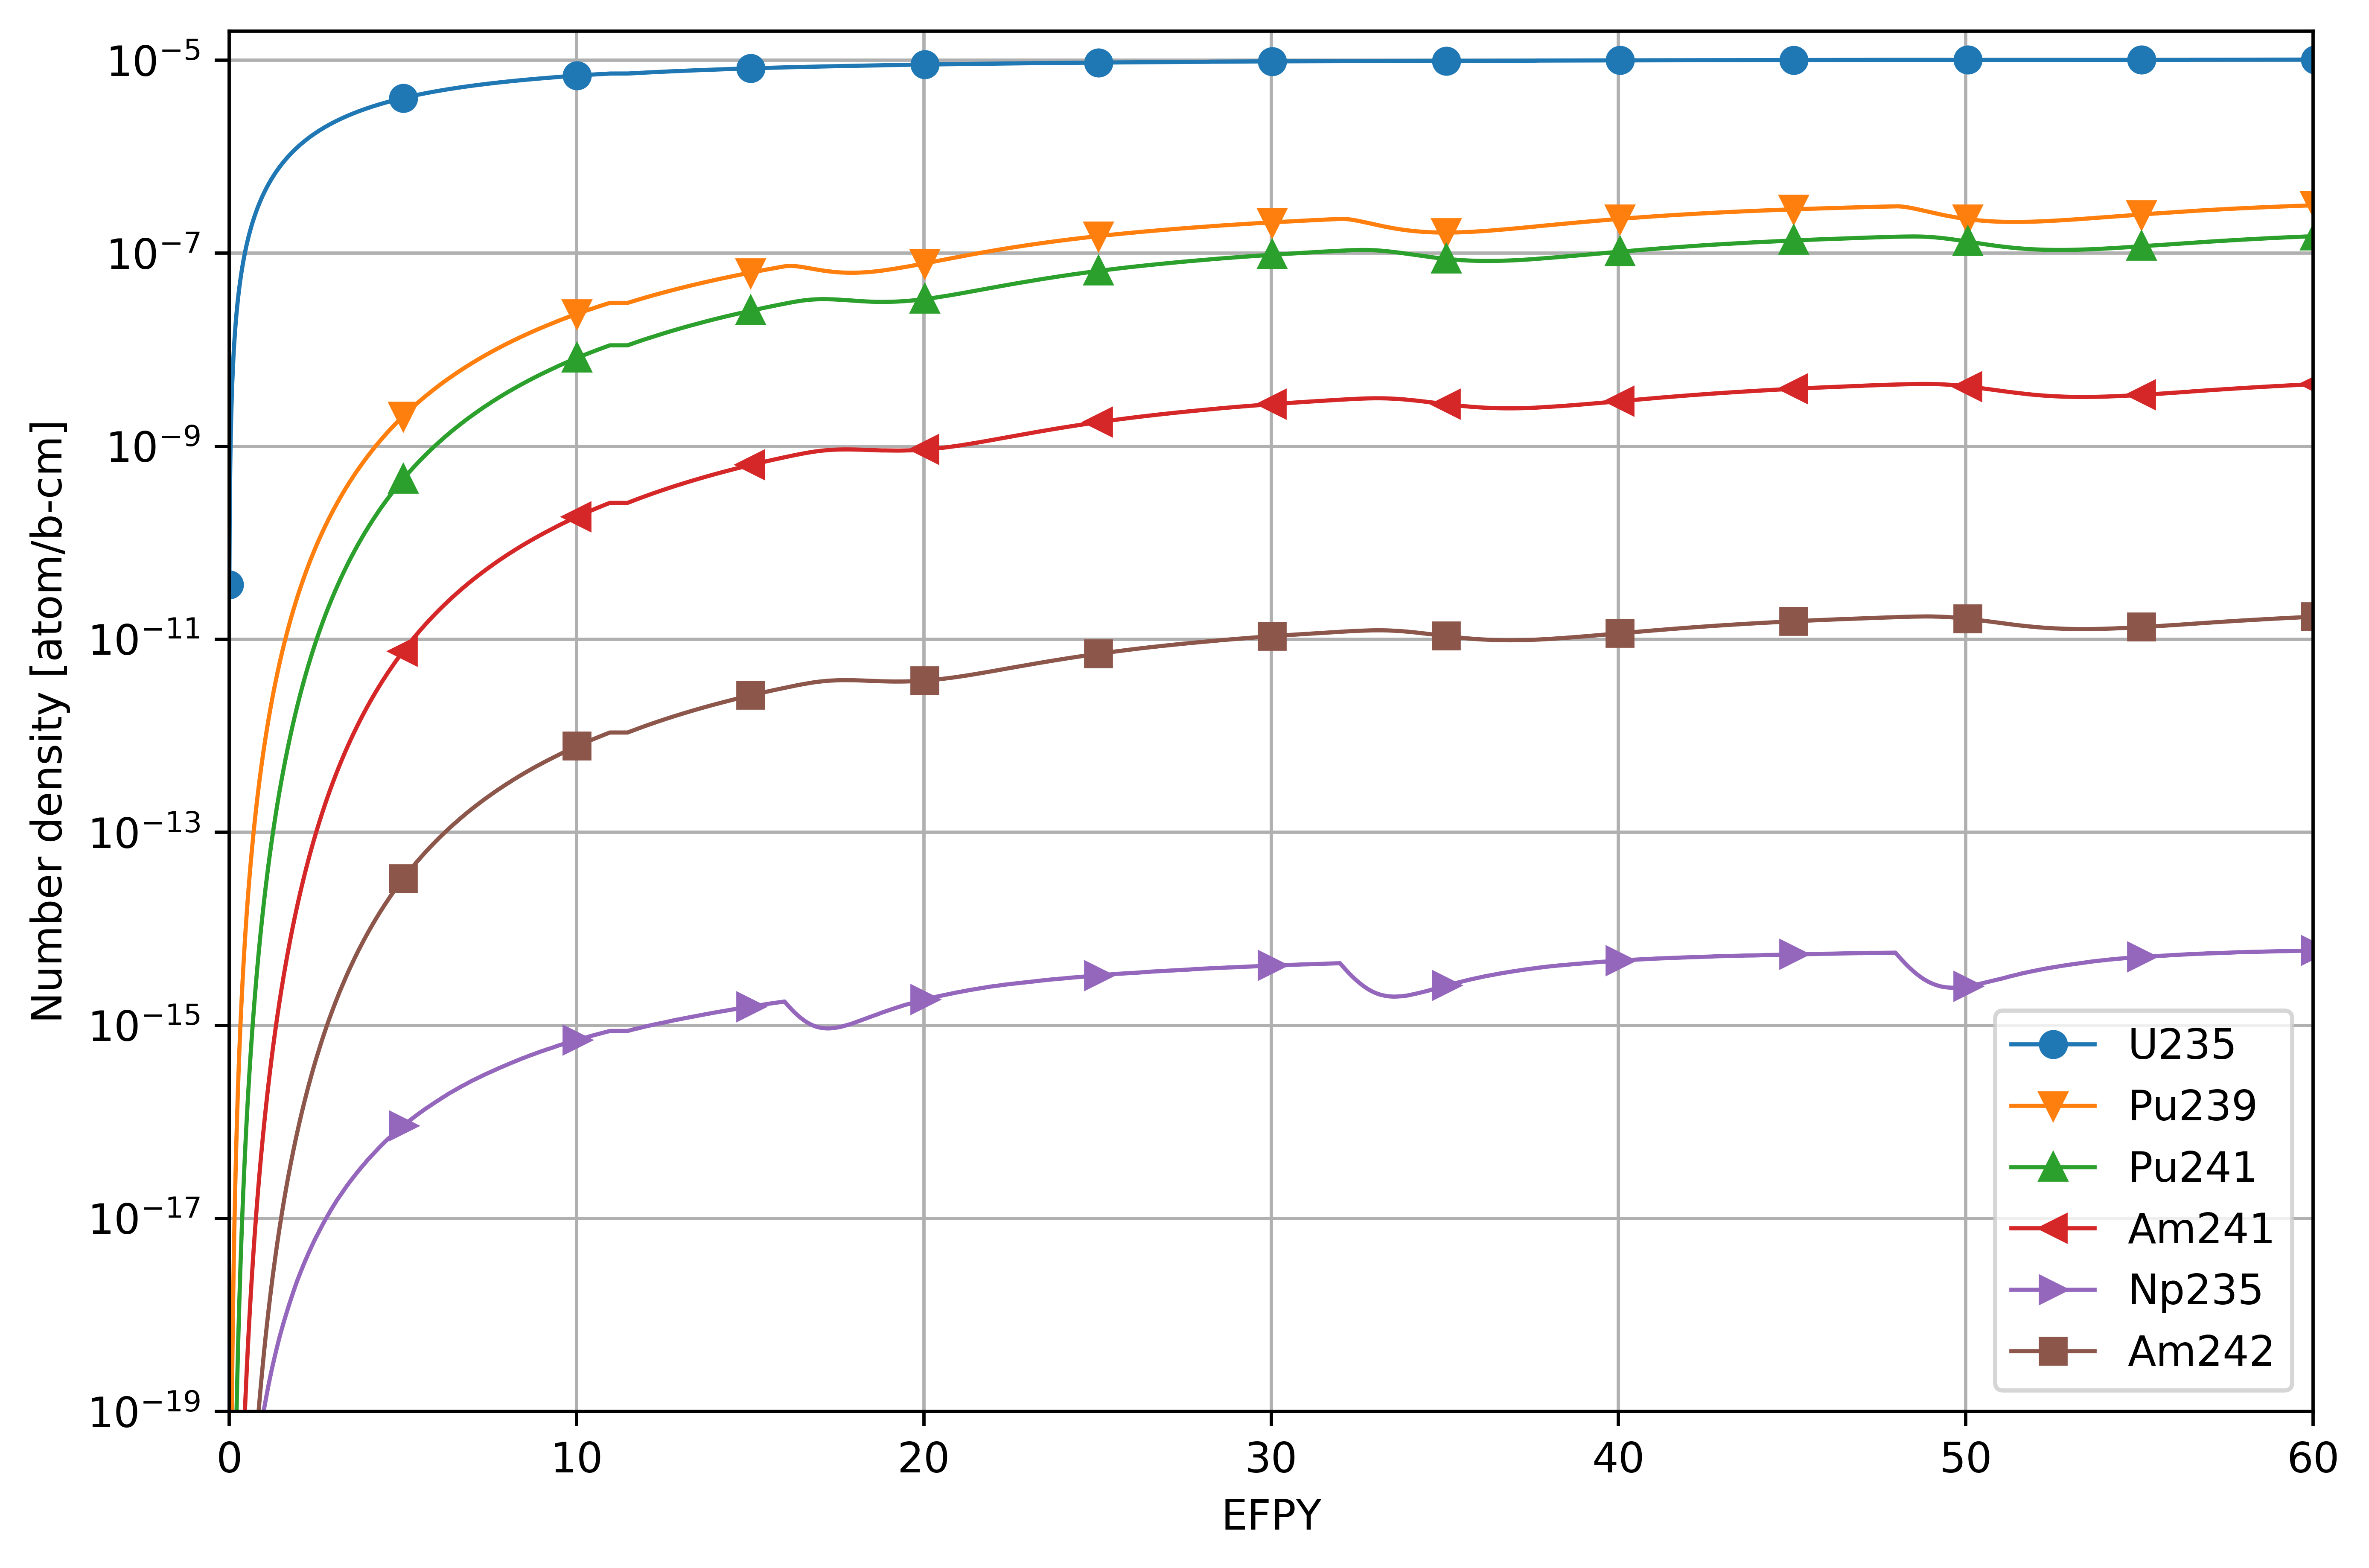
\includegraphics[width=\textwidth]{fissile_short.png}
  \caption{Number density of fissile in epithermal spectrum nuclides 
  accumulation during the reactor operation.}
  \label{fig:fissile_short}
\end{figure}

\subsection{Neutron spectrum}
Figure~\ref{fig:spectrum} shows the normalized neutron flux spectrum for the 
full-core \gls{MSBR} model in the energy range from $10^{-8}$ to $10$ MeV. The 
neutron energy spectrum at equilibrium is harder than at startup due to 
plutonium and other strong absorbers accumulation in the core during reactor 
operation.  
\begin{figure}[ht!] % replace 't' with 'b'         to force it to 
  \centering
  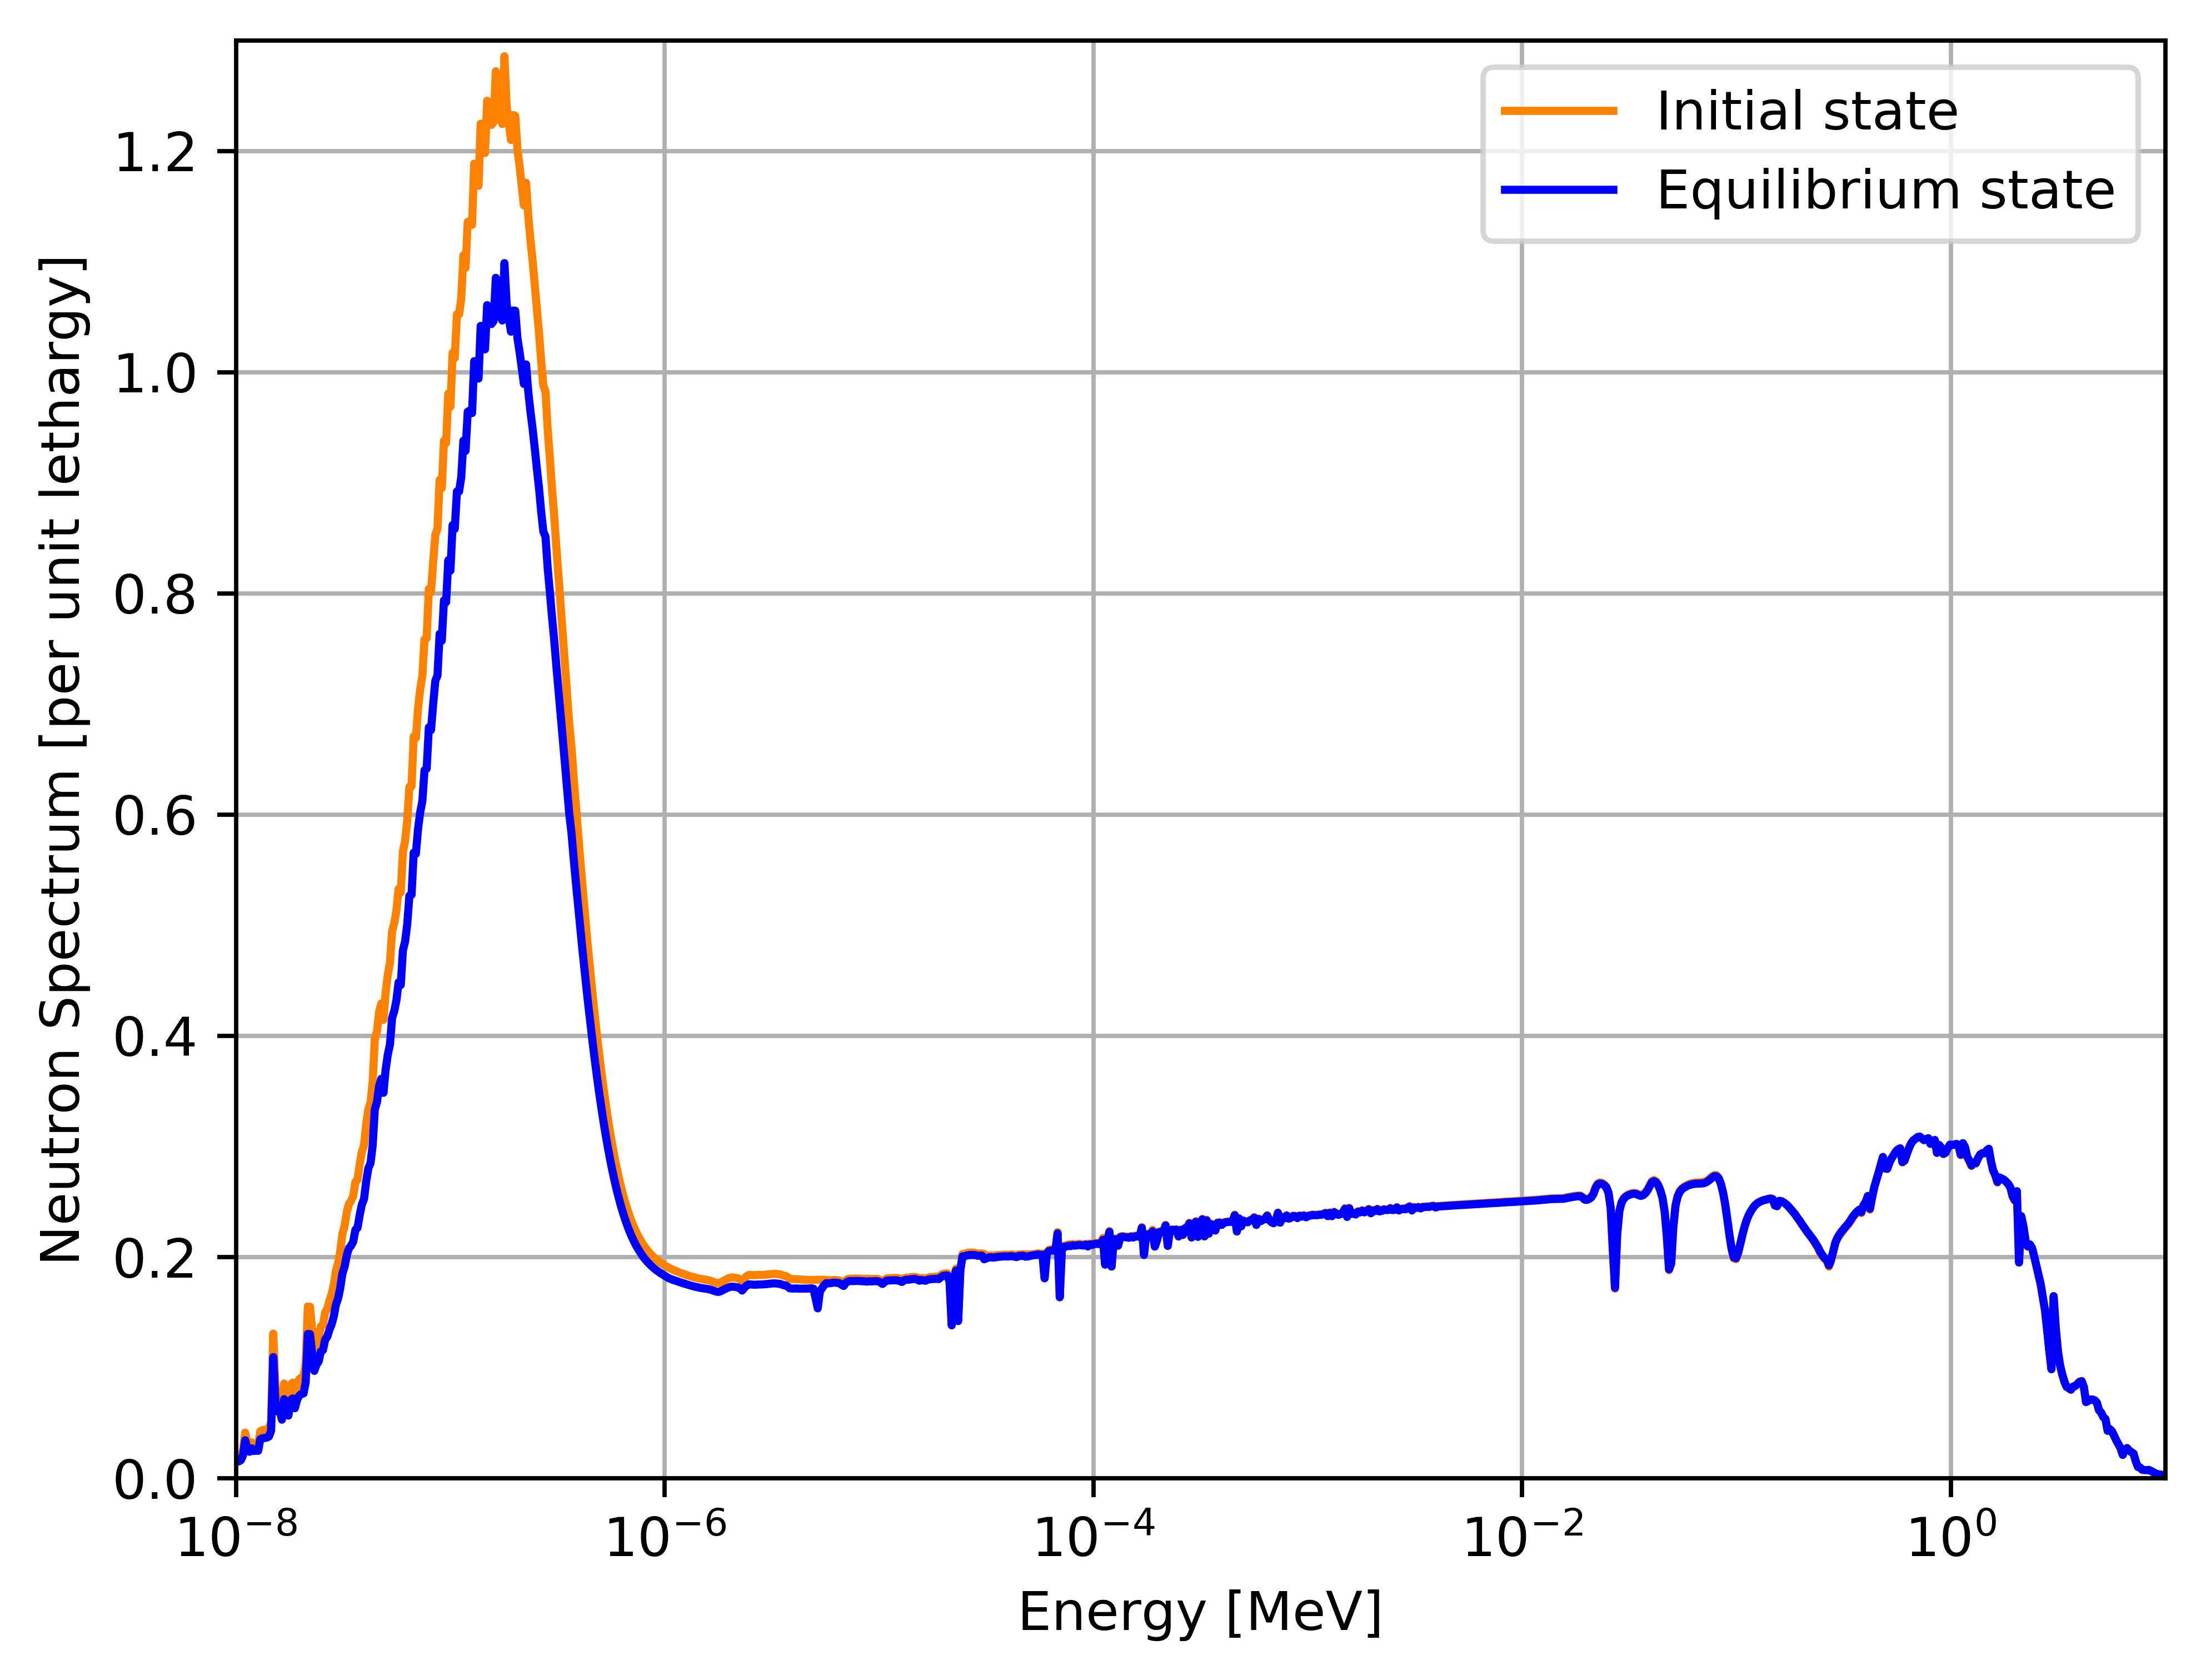
\includegraphics[width=\textwidth]{spectrum.png} \caption{Neutron flux energy 
  spectrum normalized by unit lethargy and area under the curve is normalized to 1 for initial and equilibrium fuel salt 
  composition.}
  \label{fig:spectrum}
\end{figure}

Figure~\ref{fig:spectrum_zones} shows that zone I produced more thermal neutrons 
than zone II, corresponding to a majority of fissions occurring in the central part 
of the core. In the undermoderated zone II, the neutron energy spectrum is harder, 
which leads to more neutrons capture by $^{232}$Th and helps achieve relatively 
high breeding ratio. Moreover, the (n,$\gamma$) resonance energy range in $^{232}$Th 
is from 10$^{-4}$ to 10$^{-2}$ MeV. Therefore, the moderator-to-fuel ratio for zone 
II was chosen to shift the neutron energy spectrum in this range. Furthermore, in the 
central core region (zone I), the neutron energy spectrum shifts to a harder spectrum 
over 20 years of reactor operation. Meanwhile, in the outer core region (zone II), a 
similar spectral shift takes place at a reduced scale. These results are in a good 
agreement with original ORNL report \cite{robertson_conceptual_1971} and the most recent 
whole-core steady-state study \cite{park_whole_2015}.

It is important to obtain the epithermal and thermal spectra to produce $^{233}$U from 
$^{232}$Th because the radiative capture cross section of thorium decreases monotonically 
from $10^{-10}$ MeV to $10^{-5}$ MeV. Hardening the spectrum tends to significantly 
increase resonance absorption in thorium and decrease absorptions in fissile and 
construction materials. 
\begin{figure}[ht!] % replace 't' with 'b' to force it to 
  \centering
  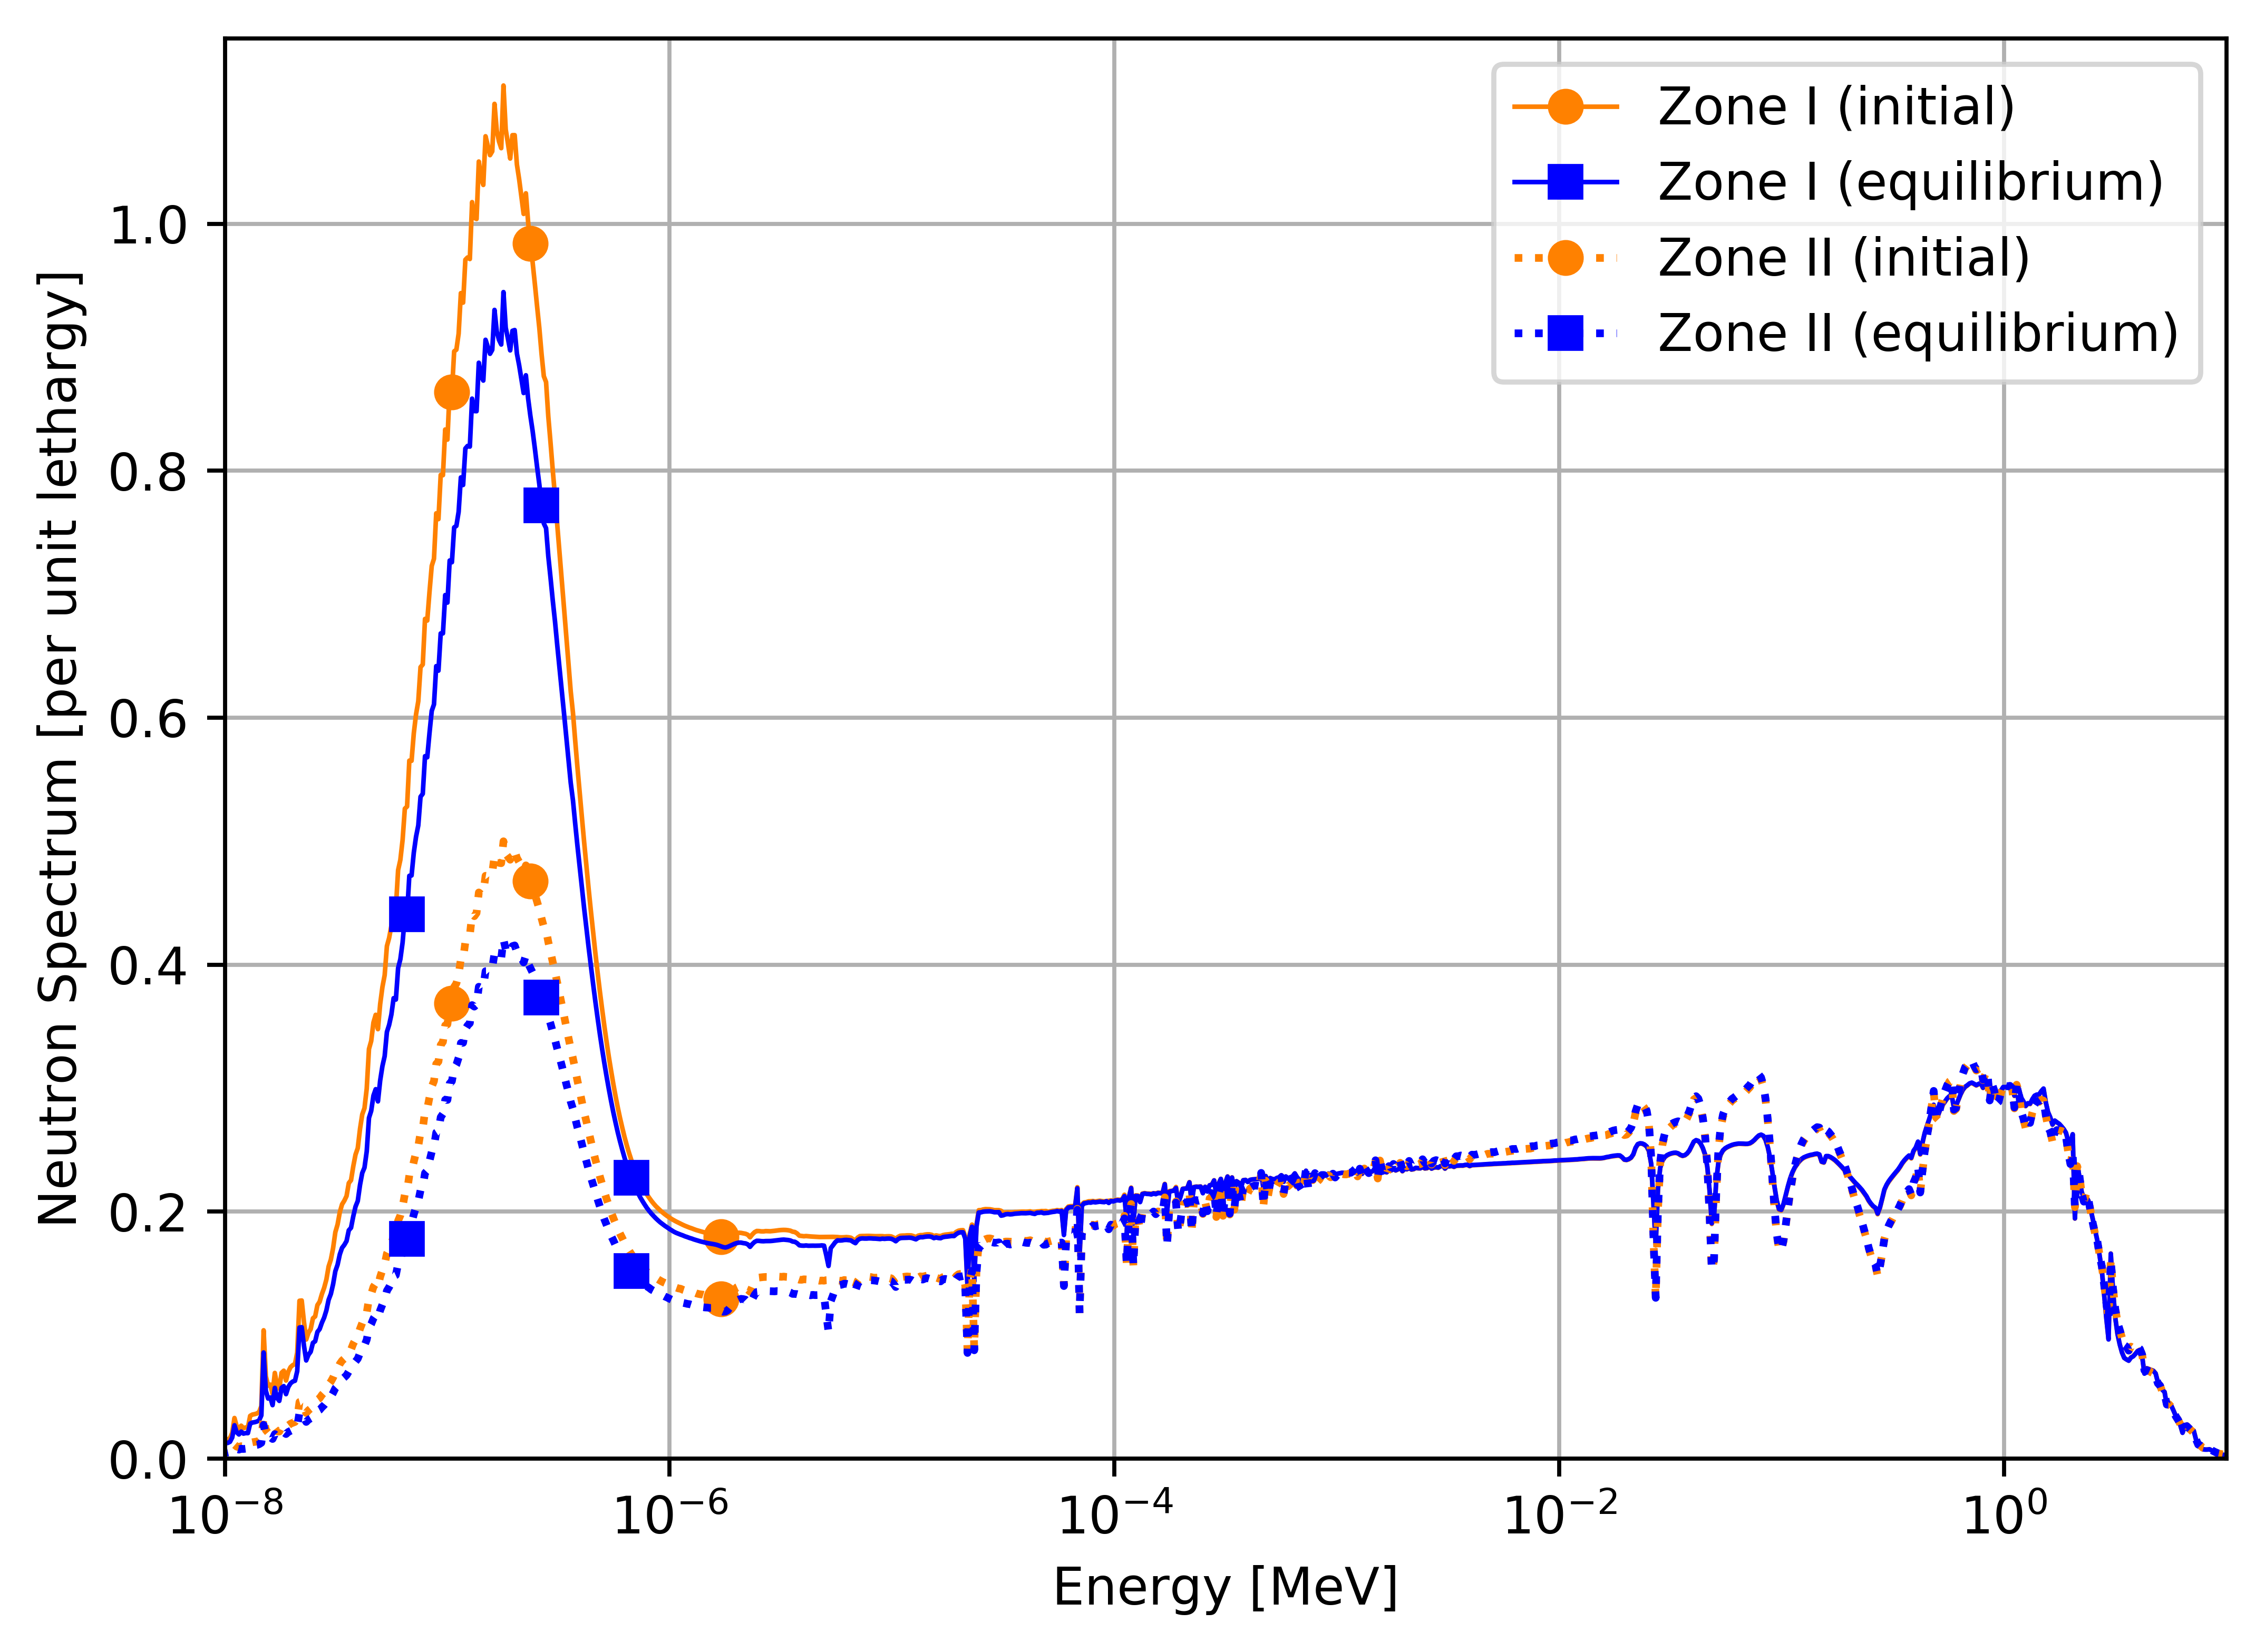
\includegraphics[width=\textwidth]{spectrum_zones.png} 
  \caption{Neutron flux energy spectrum in different core regions normalized by 
unit lethargy and area under the curve is normalized to 1 for the initial and equilibrium fuel salt composition.}
  \label{fig:spectrum_zones}
\end{figure}

\subsection{Neutron flux}
Figure~\ref{fig:radial_flux} shows the radial distribution of fast and thermal 
neutron flux for the both initial and equilibrium composition. The neutron fluxes
have similar shapes for both compositions but the equilibrium case has a harder 
spectrum. A significant spectral shift was observed in the central region of 
the core (zone I), while for the outer region (zone II), it is negligible for fast 
but notable for thermal neutrons. These neutron flux radial distributions 
agree with the fluxes in the original ORNL report \cite{robertson_conceptual_1971}. 
Overall, spectrum hardening during \gls{MSBR} operation should be carefully 
studied when designing the reactivity control system.
\begin{figure}[ht!] % replace 't' with 'b' to force it to \centering
  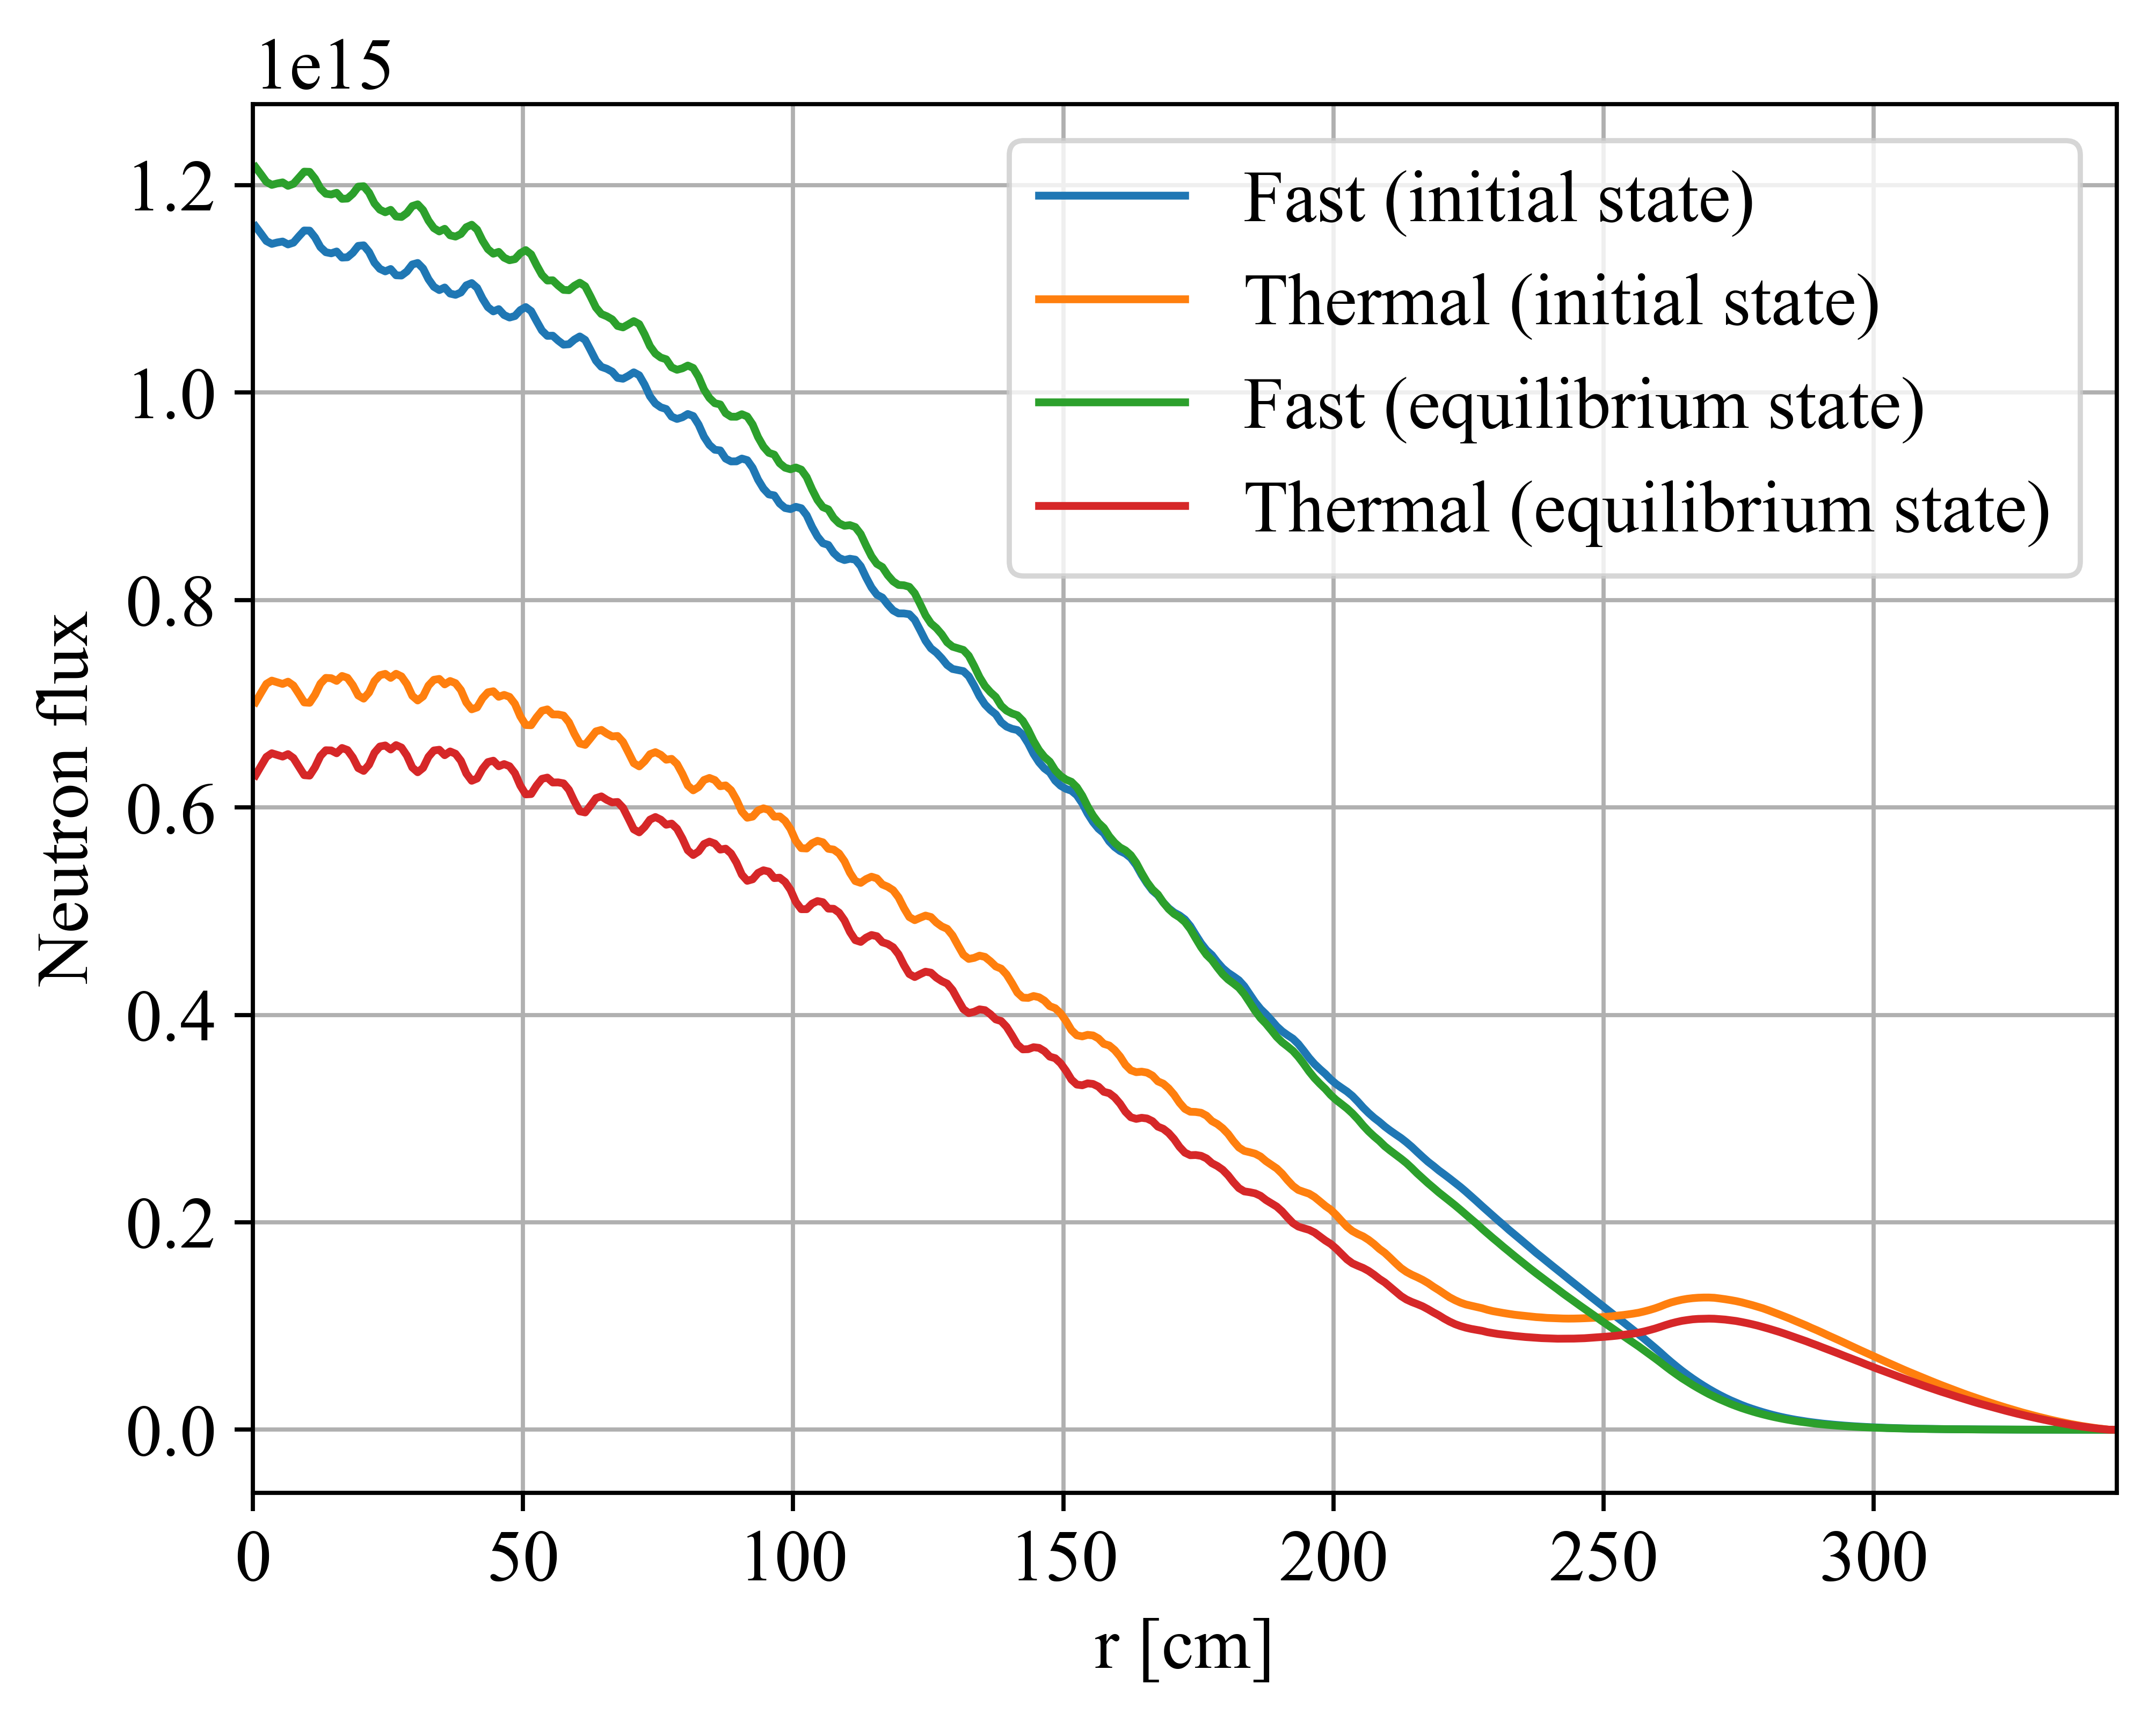
\includegraphics[width=\textwidth]{radial_flux.png} \caption{Radial neutron 
  flux distribution for initial and equilibrium fuel salt composition.}
  \label{fig:radial_flux}
\end{figure}

\subsection{Power and breeding distribution}
Table~\ref{tab:powgen_fraction}	shows the power fraction in each zone for 
initial and equilibrium fuel compositions. Figure~\ref{fig:pow_den} reflects the 
normalized power distribution of the \gls{MSBR} quarter core for equilibrium fuel
 salt composition. For both the initial and equilibrium compositions, fission 
primarily occurs in the center of the core, namely zone I. The spectral shift 
during reactor operation results in slightly different power fractions at startup and 
equilibrium, but most of the power is still generated in zone I at equilibrium 
(table~\ref{tab:powgen_fraction}. 
%%%%%%%%%%%%%%%%%%%%%%%%%%%%%%%%%%%%%%%%
\begin{table}[ht!]
  \centering
  \caption{Power generation fraction in each zone for initial and equilibrium 
  state.}
\begin{tabularx}{\textwidth}{ m | s | s } \hline
Core region      & Initial      & Equilibrium   \\   \hline
Zone I           & 97.91\%      & 98.12\%   \\
Zone II          & 2.09\%       & 1.88\%   \\ \hline
\end{tabularx}
  \label{tab:powgen_fraction}
\end{table}
%%%%%%%%%%%%%%%%%%%%%%%%%%%%%%%%%%%%%%%%%%%%%%%%%%%%%%%%%%%%%%%%%%%%%%%%%%%%%%%%
Figure~\ref{fig:breeding_den} shows the neutron capture reaction rate 
distribution for $^{232}$Th normalized by the total neutron flux for initial 
and equilibrium states. The distribution reflects the spatial distribution of 
$^{233}$U production in the core. The thorium-233 produced after $^{232}$Th 
captured neutron then $\beta$-decays to 
$^{233}$Pa, which is the precursor for $^{233}$U production. Accordingly, this 
characteristic represents the breeding distribution in the \gls{MSBR} core. 
Spectral shift does not cause significant changes in power nor in breeding 
distribution. Even after 20 years of operation, most of the power is still 
generated in zone I.
\begin{figure}[ht!] % replace 't' with 'b' to force it to \centering
  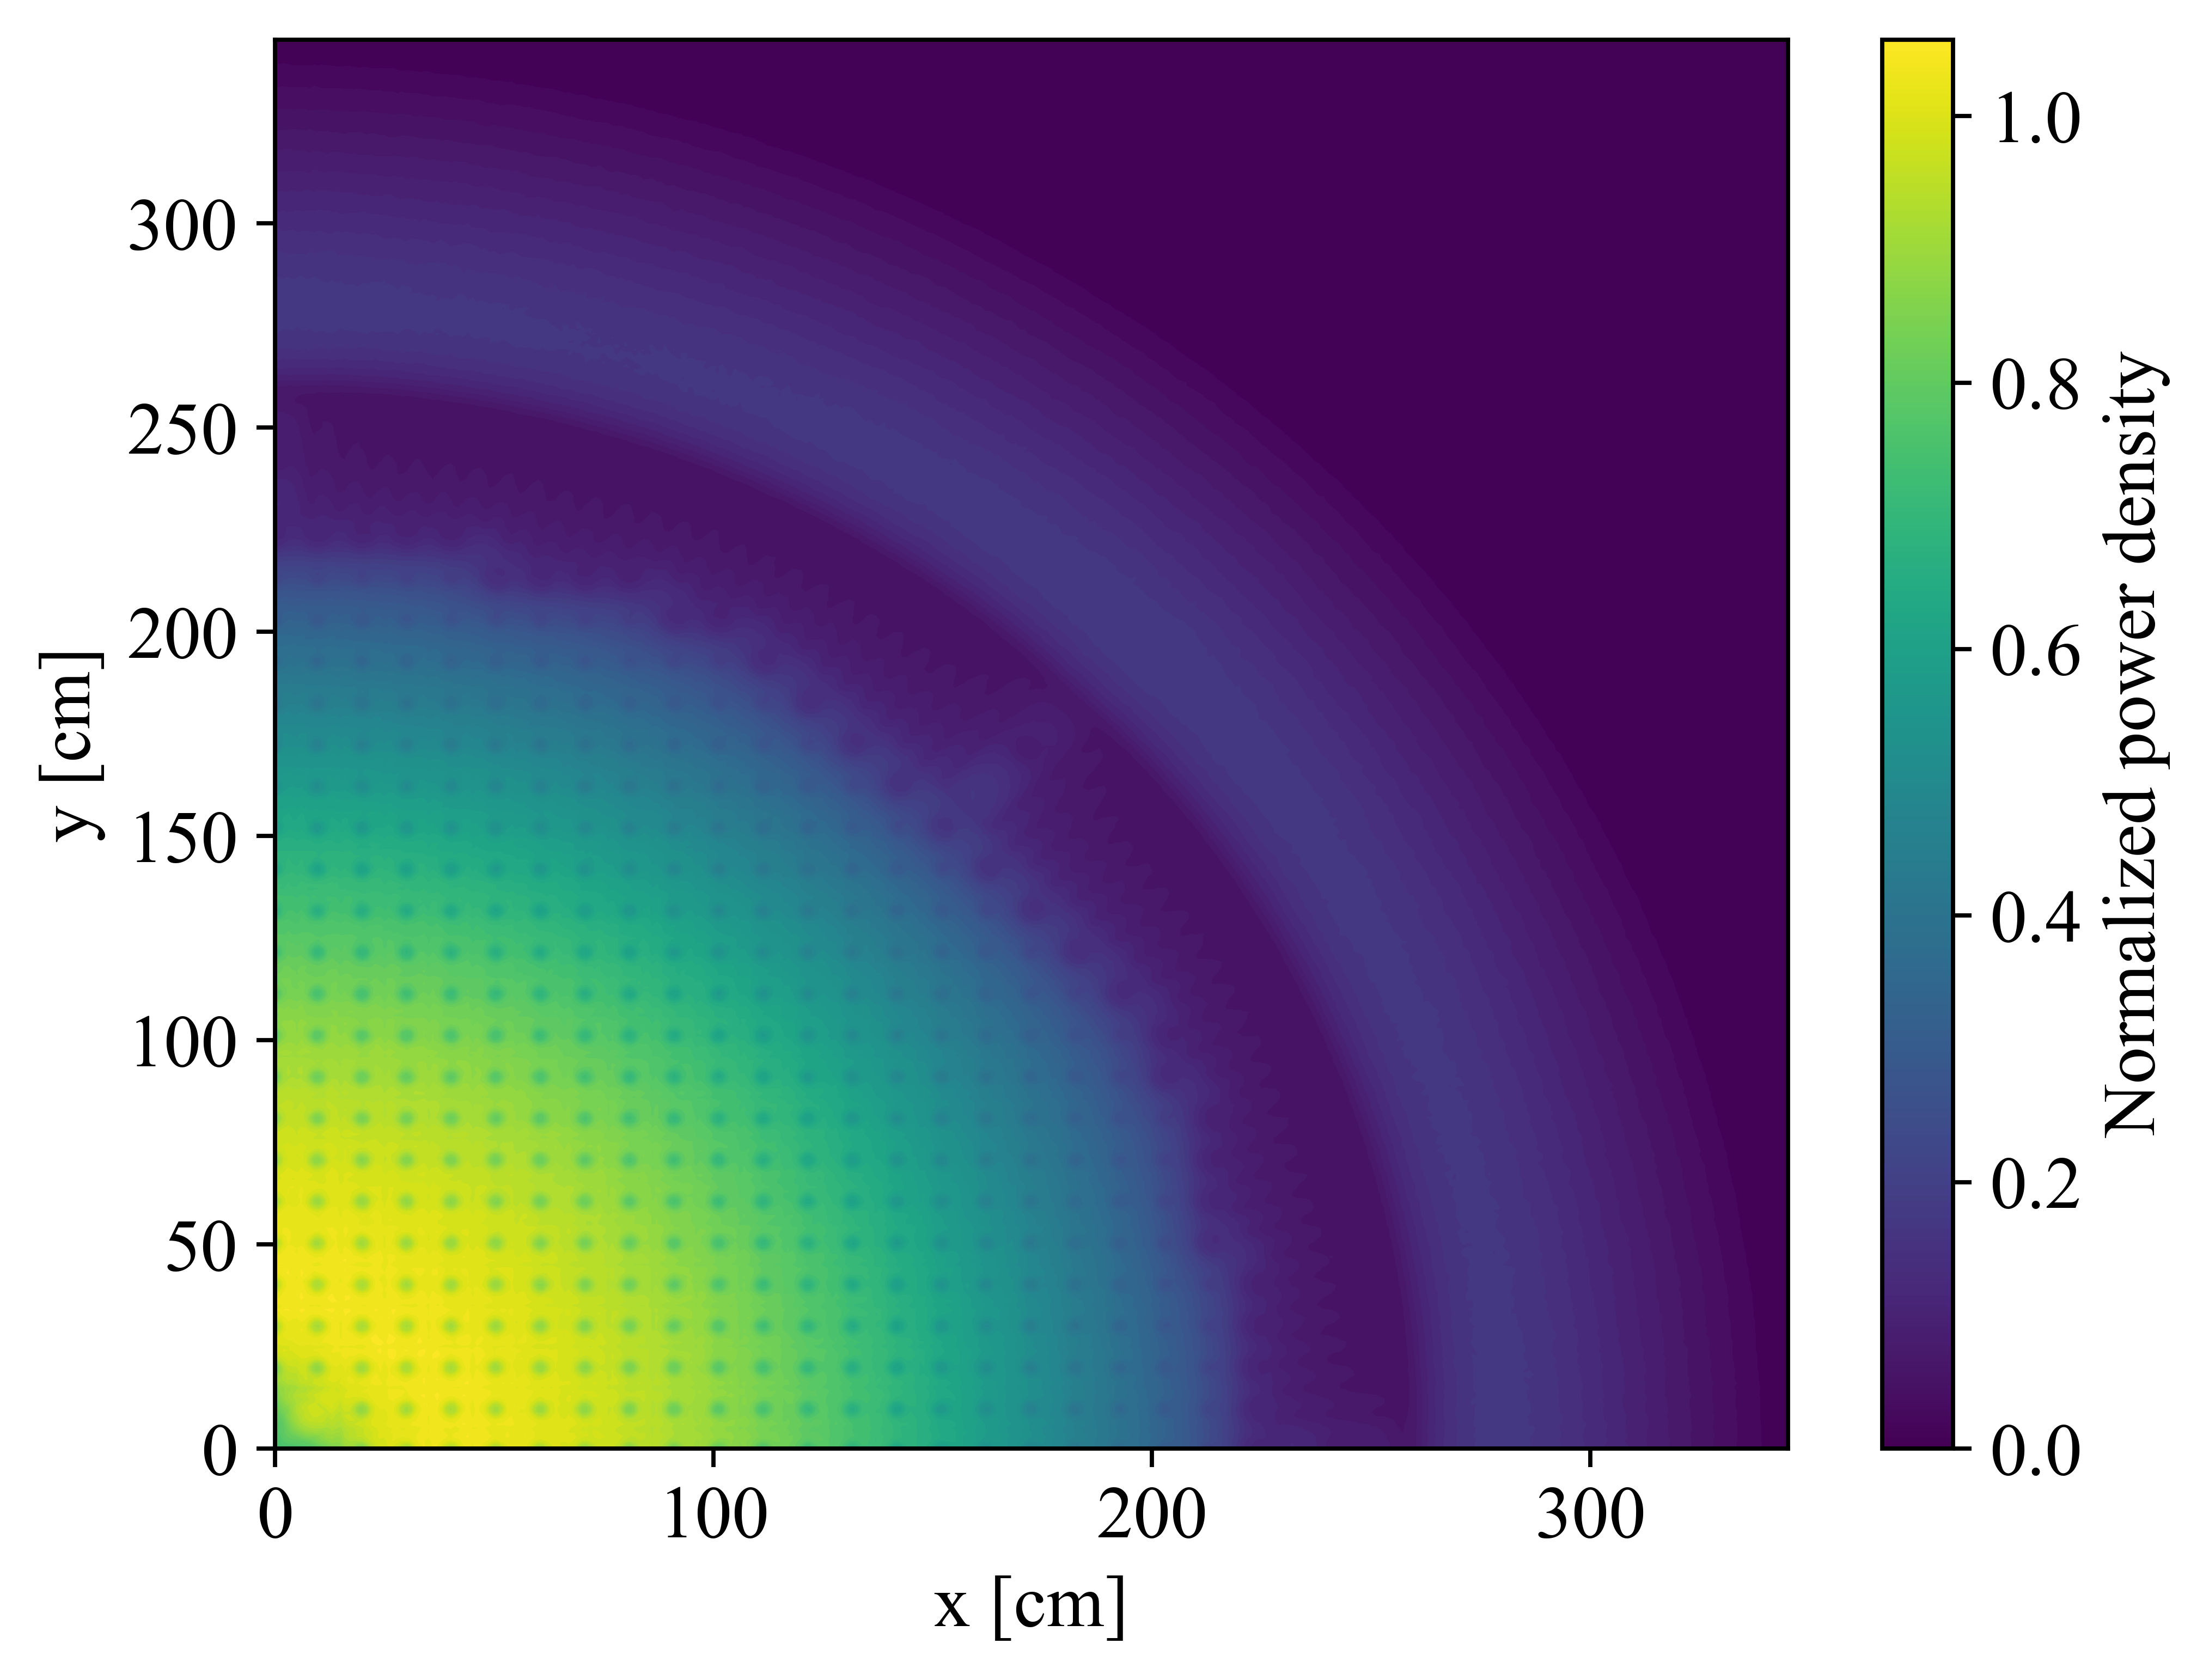
\includegraphics[width=\textwidth]{power_distribution_eq.png} 
  \caption{Normalized power density for equilibrium fuel salt 
  composition.}
  \label{fig:pow_den}
\end{figure}
\begin{figure}[ht!] % replace 't' with 'b' to force it to \centering
  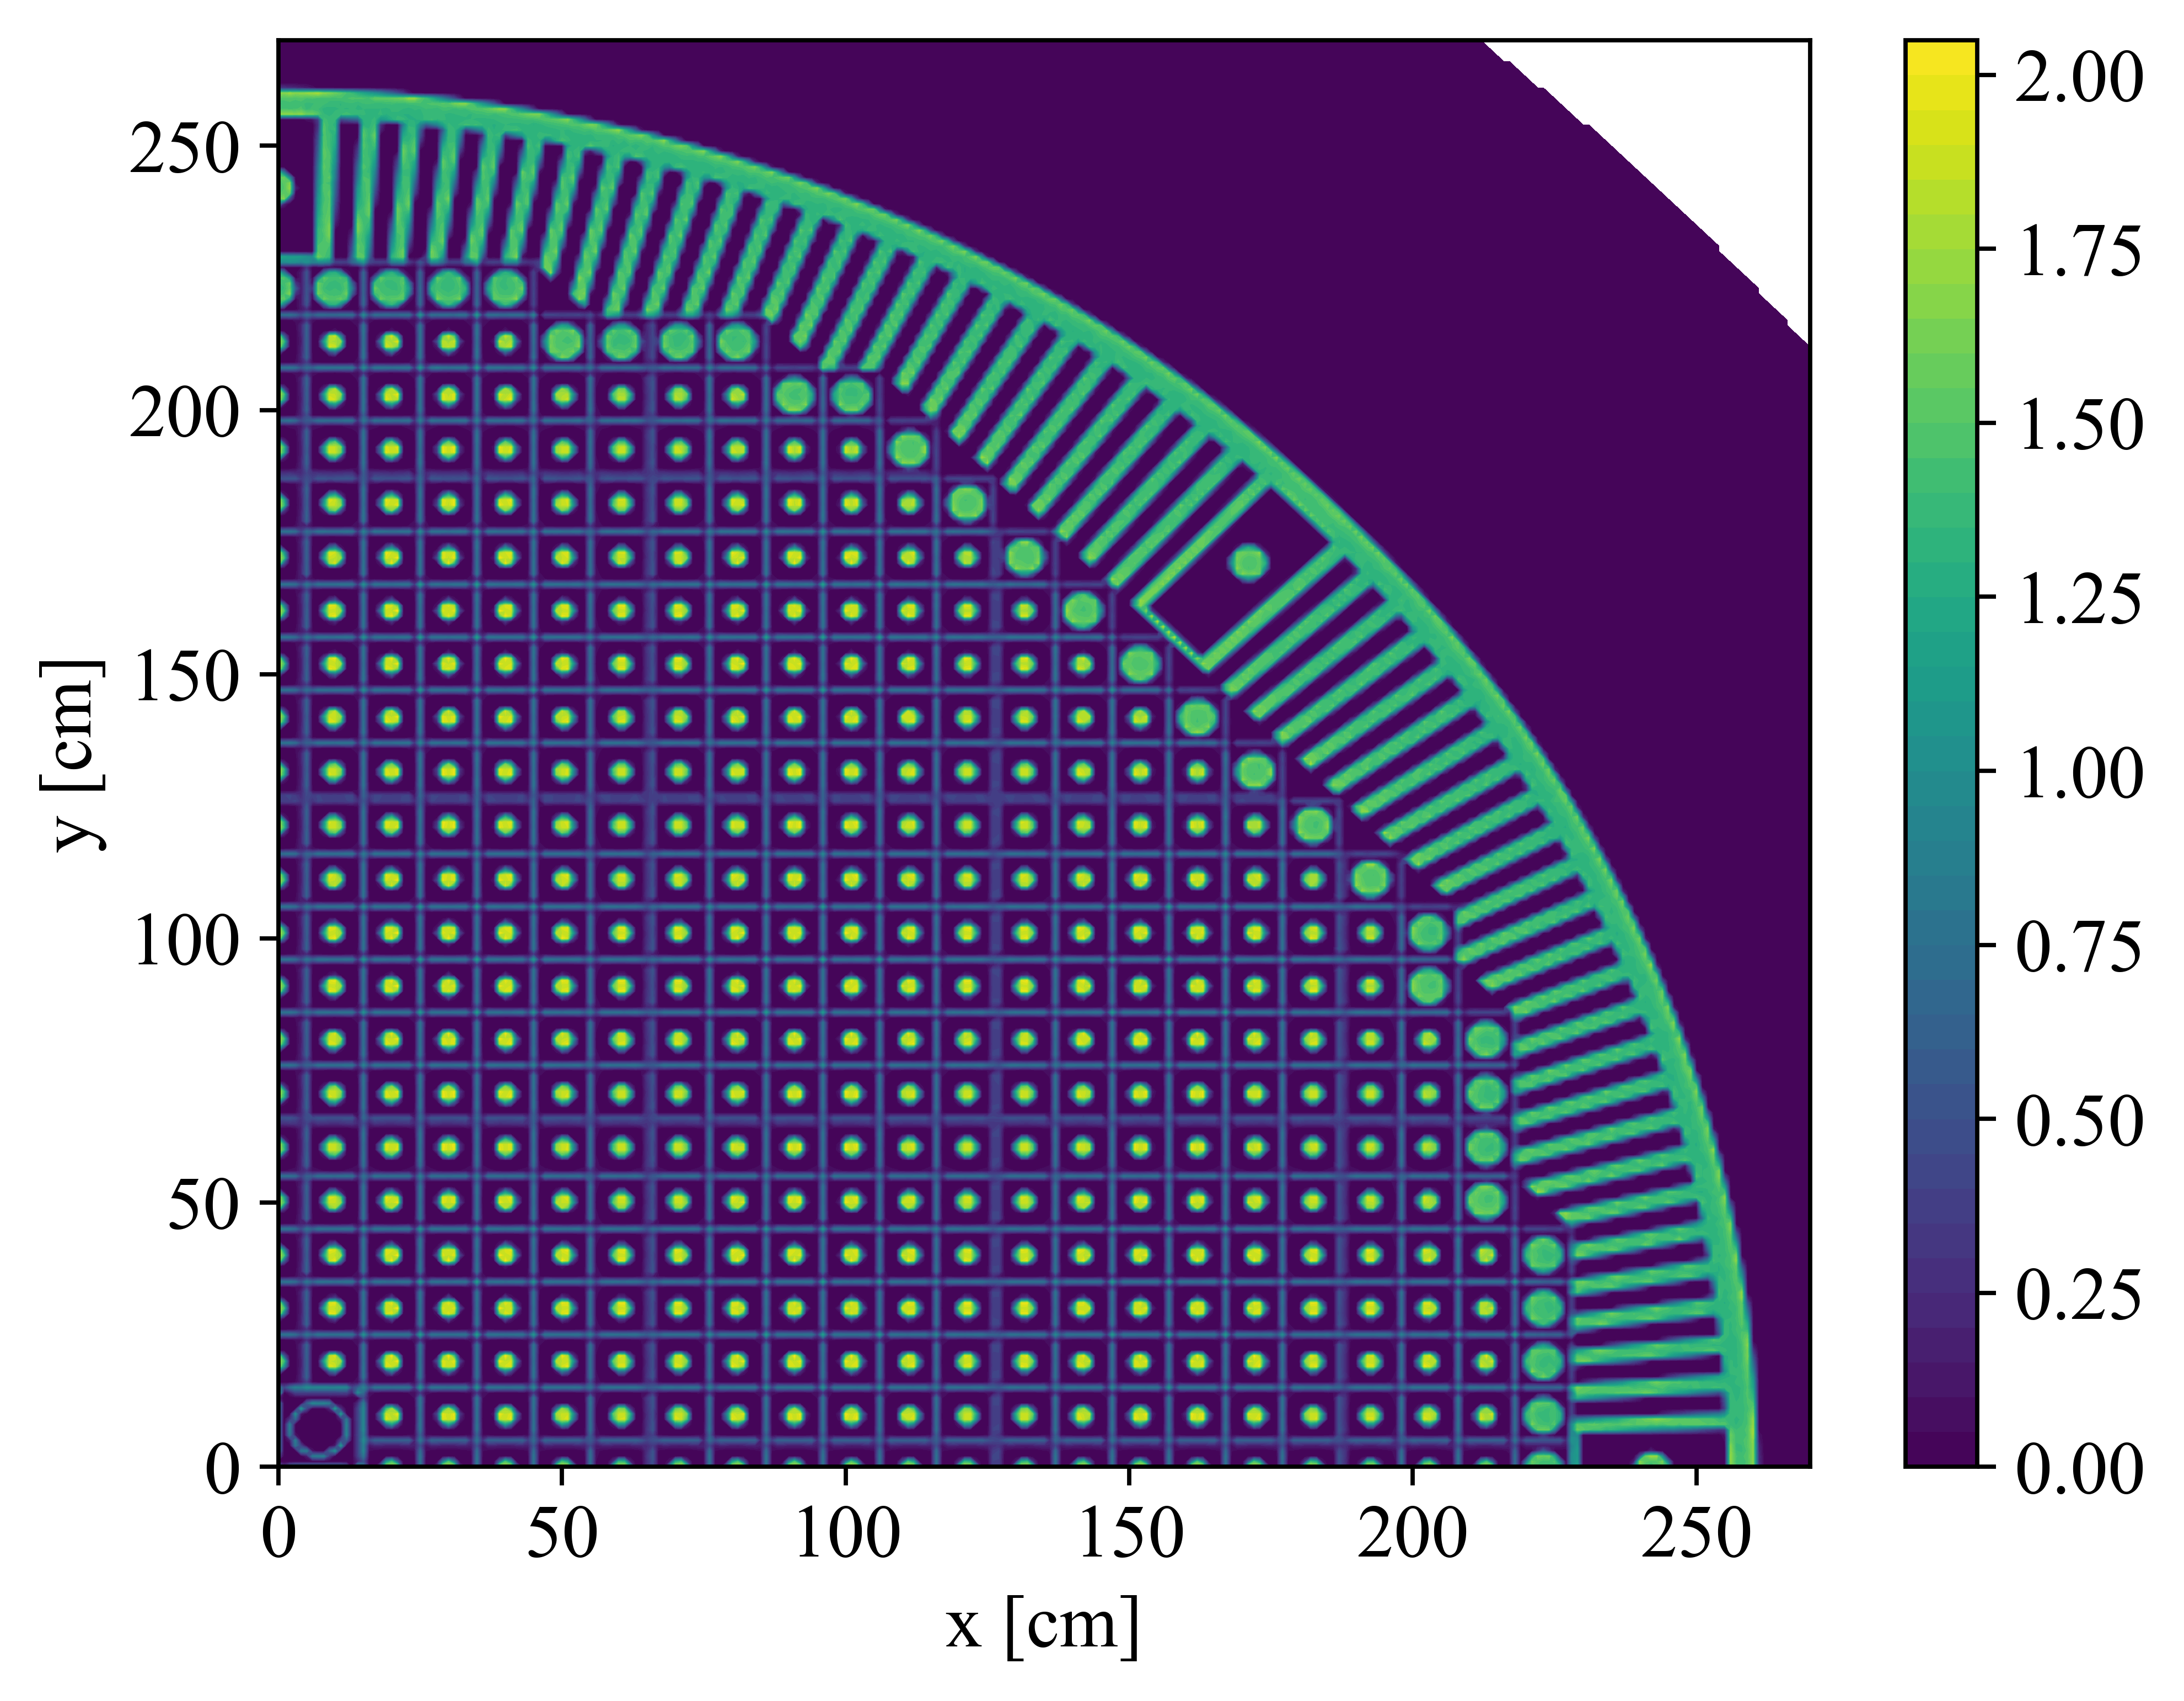
\includegraphics[width=\textwidth]{breeding_distribution_eq.png} 
  \caption{$^{232}$Th neutron capture reaction rate normalized by total flux 
  for equilibrium fuel salt composition.}
  \label{fig:breeding_den}
\end{figure}
\subsection{Temperature coefficient of reactivity}
Table~\ref{tab:tcoef} summarizes temperature effects on reactivity calculated 
in this work for both initial and equilibrium fuel compositions, compared 
with the original \gls{ORNL} report data \cite{robertson_conceptual_1971}. 
Uncertainty for each temperature coefficient was obtain by propagating statistical 
 error of effective multiplication factor calculation 
provided by SERPENT2 and also appears in 
Table~\ref{tab:tcoef}. Other sources of uncertainty, such as cross section libraries 
uncertainty, error in salt and graphite density correlations, are not treated here.
 The main physical principle underlying the reactor 
temperature feedback is an expansion of material that is heated. When the fuel 
salt temperature increases, the density of the salt decreases, but at the same 
time, the total volume of fuel salt in the core remains constant because it is 
bounded by the graphite. When the graphite temperature increases, the density 
of graphite decreases, creating additional space for fuel salt. To determine 
the temperature coefficients, the cross section temperatures for the fuel and 
moderator were changed from 900K to 1000K. Three different cases were considered:
\begin{enumerate}
  \item Temperature of fuel salt rising from 900K to 1000K.
  \item Temperature of graphite rising from 900K to 1000K.
  \item Whole reactor temperature rising from 900K to 1000K.
\end{enumerate}
%%%%%%%%%%%%%%%%%%%%%%%%%%%%%%%%%%%%%%%%
\begin{table}[ht!]
  \centering
  \caption{Temperature coefficients of reactivity for initial and equilibrium 
  state.}
\begin{tabularx}{\textwidth}{ m | s | s | x } \hline
   Reactivity coefficient [pcm/K]  & Initial      & Equilibrium  & Reference \qquad (initial)\cite{robertson_conceptual_1971} \\  \hline
Doppler in fuel salt   			& $-4.73\pm0.038$ & $-4.69\pm0.038$ & $-4.37$  \\
Fuel salt density      			& $+1.21\pm0.038$ & $+1.66\pm0.038$ & $+1.09$  \\
Total fuel salt        			& $-3.42\pm0.038$ & $-2.91\pm0.038$ & $-3.22$  \\ \hline
Graphite spectral shift    		& $+1.56\pm0.038$ & $+1.27\pm0.038$ &          \\
Graphite density   				& $+0.14\pm0.038$ & $+0.23\pm0.038$ &          \\
Total moderator (graphite)		& $+1.69\pm0.038$ & $+1.35\pm0.038$ & $+2.35$  \\ \hline
Total core      				& $-1.64\pm0.038$ & $-1.58\pm0.038$ & $-0.87$  \\ \hline
\end{tabularx}
  \label{tab:tcoef}
\end{table}
%%%%%%%%%%%%%%%%%%%%%%%%%%%%%%%%%%%%%%%%%%%%%%%%%%%%%%%%%%%%%%%%%%%%%%%%%%%%%%%%
In the first case, changes in the fuel temperature only impact fuel density. In 
this case, the geometry is unchanged because the fuel is a liquid. However, 
when the moderator heats up, both the density and the geometry change due to 
thermal expansion of the solid graphite blocks and reflector. Accordingly, the 
new graphite density was calculated using a linear temperature expansion 
coefficient of 1.3$\times10^{-6}$K$^{-1}$ \cite{robertson_conceptual_1971}. A new 
geometry input for SERPENT2, which takes into account displacement of graphite 
surfaces, was created based on this information. For the displacements calculation 
it was assumed that the interface between graphite reflector and vessel did not move,
 and the vessel temperature did not change. This is the most reasonable assumption for
 the short-term reactivity effects because inlet salt is cooling graphite reflector and 
inner surface of the vessel.

The fuel temperature coefficient (FTC) is negative for both initial and 
equilibrium fuel compositions due to thermal Doppler broadening of the resonance 
capture cross sections in the thorium. Small positive effect of fuel density on 
reactivity is increasing from +1.21 pcm/K for the reactor startup to +1.66 pcm/K for 
equilibrium fuel composition which has negative effect on FTC magnitude during the 
reactor operation. This is in good agreement with earlier 
research \cite{robertson_conceptual_1971,park_whole_2015}. The moderator 
temperature coefficient (MTC) is positive for the startup composition and decreases 
during reactor operation because of spectrum hardening with fuel depletion. 
Finally, the total temperature coefficient of reactivity is negative for both 
cases, but decreases during reactor operation due to spectral shift. In 
summary, even after 20 years of operation the total temperature coefficient of 
reactivity is relatively large and negative during reactor operation (comparing 
with conventional PWR which has temperature coefficient about -1.71 pcm/$^\circ$F 
$\approx$ -3.08 pcm/K \cite{forget_integral_2018}), despite positive MTC, and 
affords excellent reactor stability and control.

\subsection{Reactivity control system rod worth}
Table~\ref{tab:rod_worth} summarizes the reactivity control system worth. 
During normal operation, the control (graphite) rods are fully inserted, and the 
safety (B$_4$C) rods are fully withdrawn. To insert negative reactivity into 
the core, the graphite rods are gradually withdrawn from the core. In an 
accident, the safety rods would be dropped down into the core. The integral rod 
worths were calculated for various positions to separately estimate the worth
of the control graphite rods\footnote{In \cite{robertson_conceptual_1971}, the 
graphite rods are referred to as ``control'' rods.}, the safety (B$_4$C) rods, 
and the whole reactivity control system. Control rod integral worth is 
approximately 28 cents and stays almost constant during reactor operation. The 
safety rod integral worth decreases by  16.2\% during 20 years of operation 
because of neutron spectrum hardening and absorber accumulation in proximity to 
reactivity control system rods. This 16\% decline in control system worth 
should be taken into account in \gls{MSBR} accident analysis and safety 
justification.
%%%%%%%%%%%%%%%%%%%%%%%%%%%%%%%%%%%%%%%%
\begin{table}[ht!]
  \centering
  \caption{Control system rod worth for initial and equilibrium fuel 
  composition.}
\begin{tabularx}{\textwidth}{ b | x | x } \hline
Reactivity parameter [cents]  &  Initial      &  Equilibrium      \\ \hline
Control (graphite) rod integral worth               & $\ 28.2\pm0.8$    & $\ 
        29.0\pm0.8$ \\ Safety (B$_4$C) rod integral worth                  & 
        $251.8\pm0.8$    & $211.0\pm0.8$  \\
Total reactivity control system worth               & $505.8\pm0.7$    & 
        $424.9\pm0.8$ \\ \hline
\end{tabularx}
  \label{tab:rod_worth}
\end{table}
%%%%%%%%%%%%%%%%%%%%%%%%%%%%%%%%%%%%%%%%%%%%%%%%%%%%%%%%%%%%%%%%%%%%%%%%%%%%%%%%

\subsection{Six Factor Analysis}
The effective multiplication factor can be expressed using the following formula:
\begin{align*}
k_{eff} = k_{inf} P_f  P_t = \eta \epsilon p f P_f P_t
\end{align*}

Table~\ref{tab:six_factor} summarizes the six factors for both initial and 
equilibrium fuel salt composition. These factors and their statistical uncertainties
 have been calculated using SERPENT2 code for initial fuel salt composition (see 
Table~\ref{tab:msbr_tab}) and for equilibrium salt composition which was obtained 
with SaltProc. The non-leakage probability for both fast 
and thermal neutrons does not change during reactor operation because these 
values are not largely affected by the neutron spectrum shift. In contrast, 
neutron reproduction factor ($\eta$), resonance escape probability (p), and 
fast fission factor ($\epsilon$) are considerably different between startup and 
equilibrium. As indicated in Figure~\ref{fig:spectrum}, the neutron spectrum is 
softer at the beginning of reactor life. Neutron spectrum hardening causes the fast 
fission factor to increase through the core lifetime. The opposite is true for the 
resonance escape probability. Finally, the neutron reproduction factor 
decreases during reactor operation due to accumulation of fissile plutonium 
isotopes.
%%%%%%%%%%%%%%%%%%%%%%%%%%%%%%%%%%%%%%%%
\begin{table}[hb!]
  \centering
  \caption{Six factors for the full-core \gls{MSBR} model for initial and 
  equilibrium fuel composition.}
\begin{tabularx}{\textwidth}{ b | s | s } \hline
Factor  & Initial      & Equilibrium   \\ \hline
Neutron reproduction factor ($\eta$)     & $1.3960\pm.000052$     & 
        $1.3778\pm.00005$ \\ Thermal utilization factor (f)           & 
        $0.9670\pm.000011$     & $0.9706\pm.00001$ \\
Resonance escape probability (p)         & $0.6044\pm.000039$     & 
        $0.5761\pm.00004$ \\
Fast fission factor ($\epsilon$)         & $1.3421\pm.000040$     & 
        $1.3609\pm.00004$ \\
Fast non-leakage probability (P$_f$)     & $0.9999\pm.000004$     & 
        $0.9999\pm.000004$ \\
Thermal non-leakage probability (P$_t$)  & $0.9894\pm.000005$     & 
        $0.9912\pm.00005$ \\ \hline
\end{tabularx}
  \label{tab:six_factor}
\end{table}
%%%%%%%%%%%%%%%%%%%%%%%%%%%%%%%%%%%%%%%%%%%%%%%%%%%%%%%%%%%%%%%%%%%%%%%%%%%%%%%%
\subsection{Thorium refill rate}
In a \gls{MSBR} reprocessing scheme, the only external feed material flow  is 
$^{232}$Th. Figure~\ref{fig:th_refill} shows the $^{232}$Th feed rate 
calculated for 60 years of reactor operation. The $^{232}$Th feed rate 
fluctuates significantly as a result of the batch-wise nature of this online 
reprocessing approach. For example, the large spikes of up to 36 kg/day in a 
thorium consumption occurs every 3435 days. This is required due to batch-wise 
removal of strong absorbers (Rb, Sr, Cs, Ba). The corresponding effective 
multiplication factor increase (Figure~\ref{fig:keff}) and breeding 
intensification leads to additional $^{232}$Th consumption.  
\begin{figure}[ht!] % replace 't' with 'b' to force it to \centering
  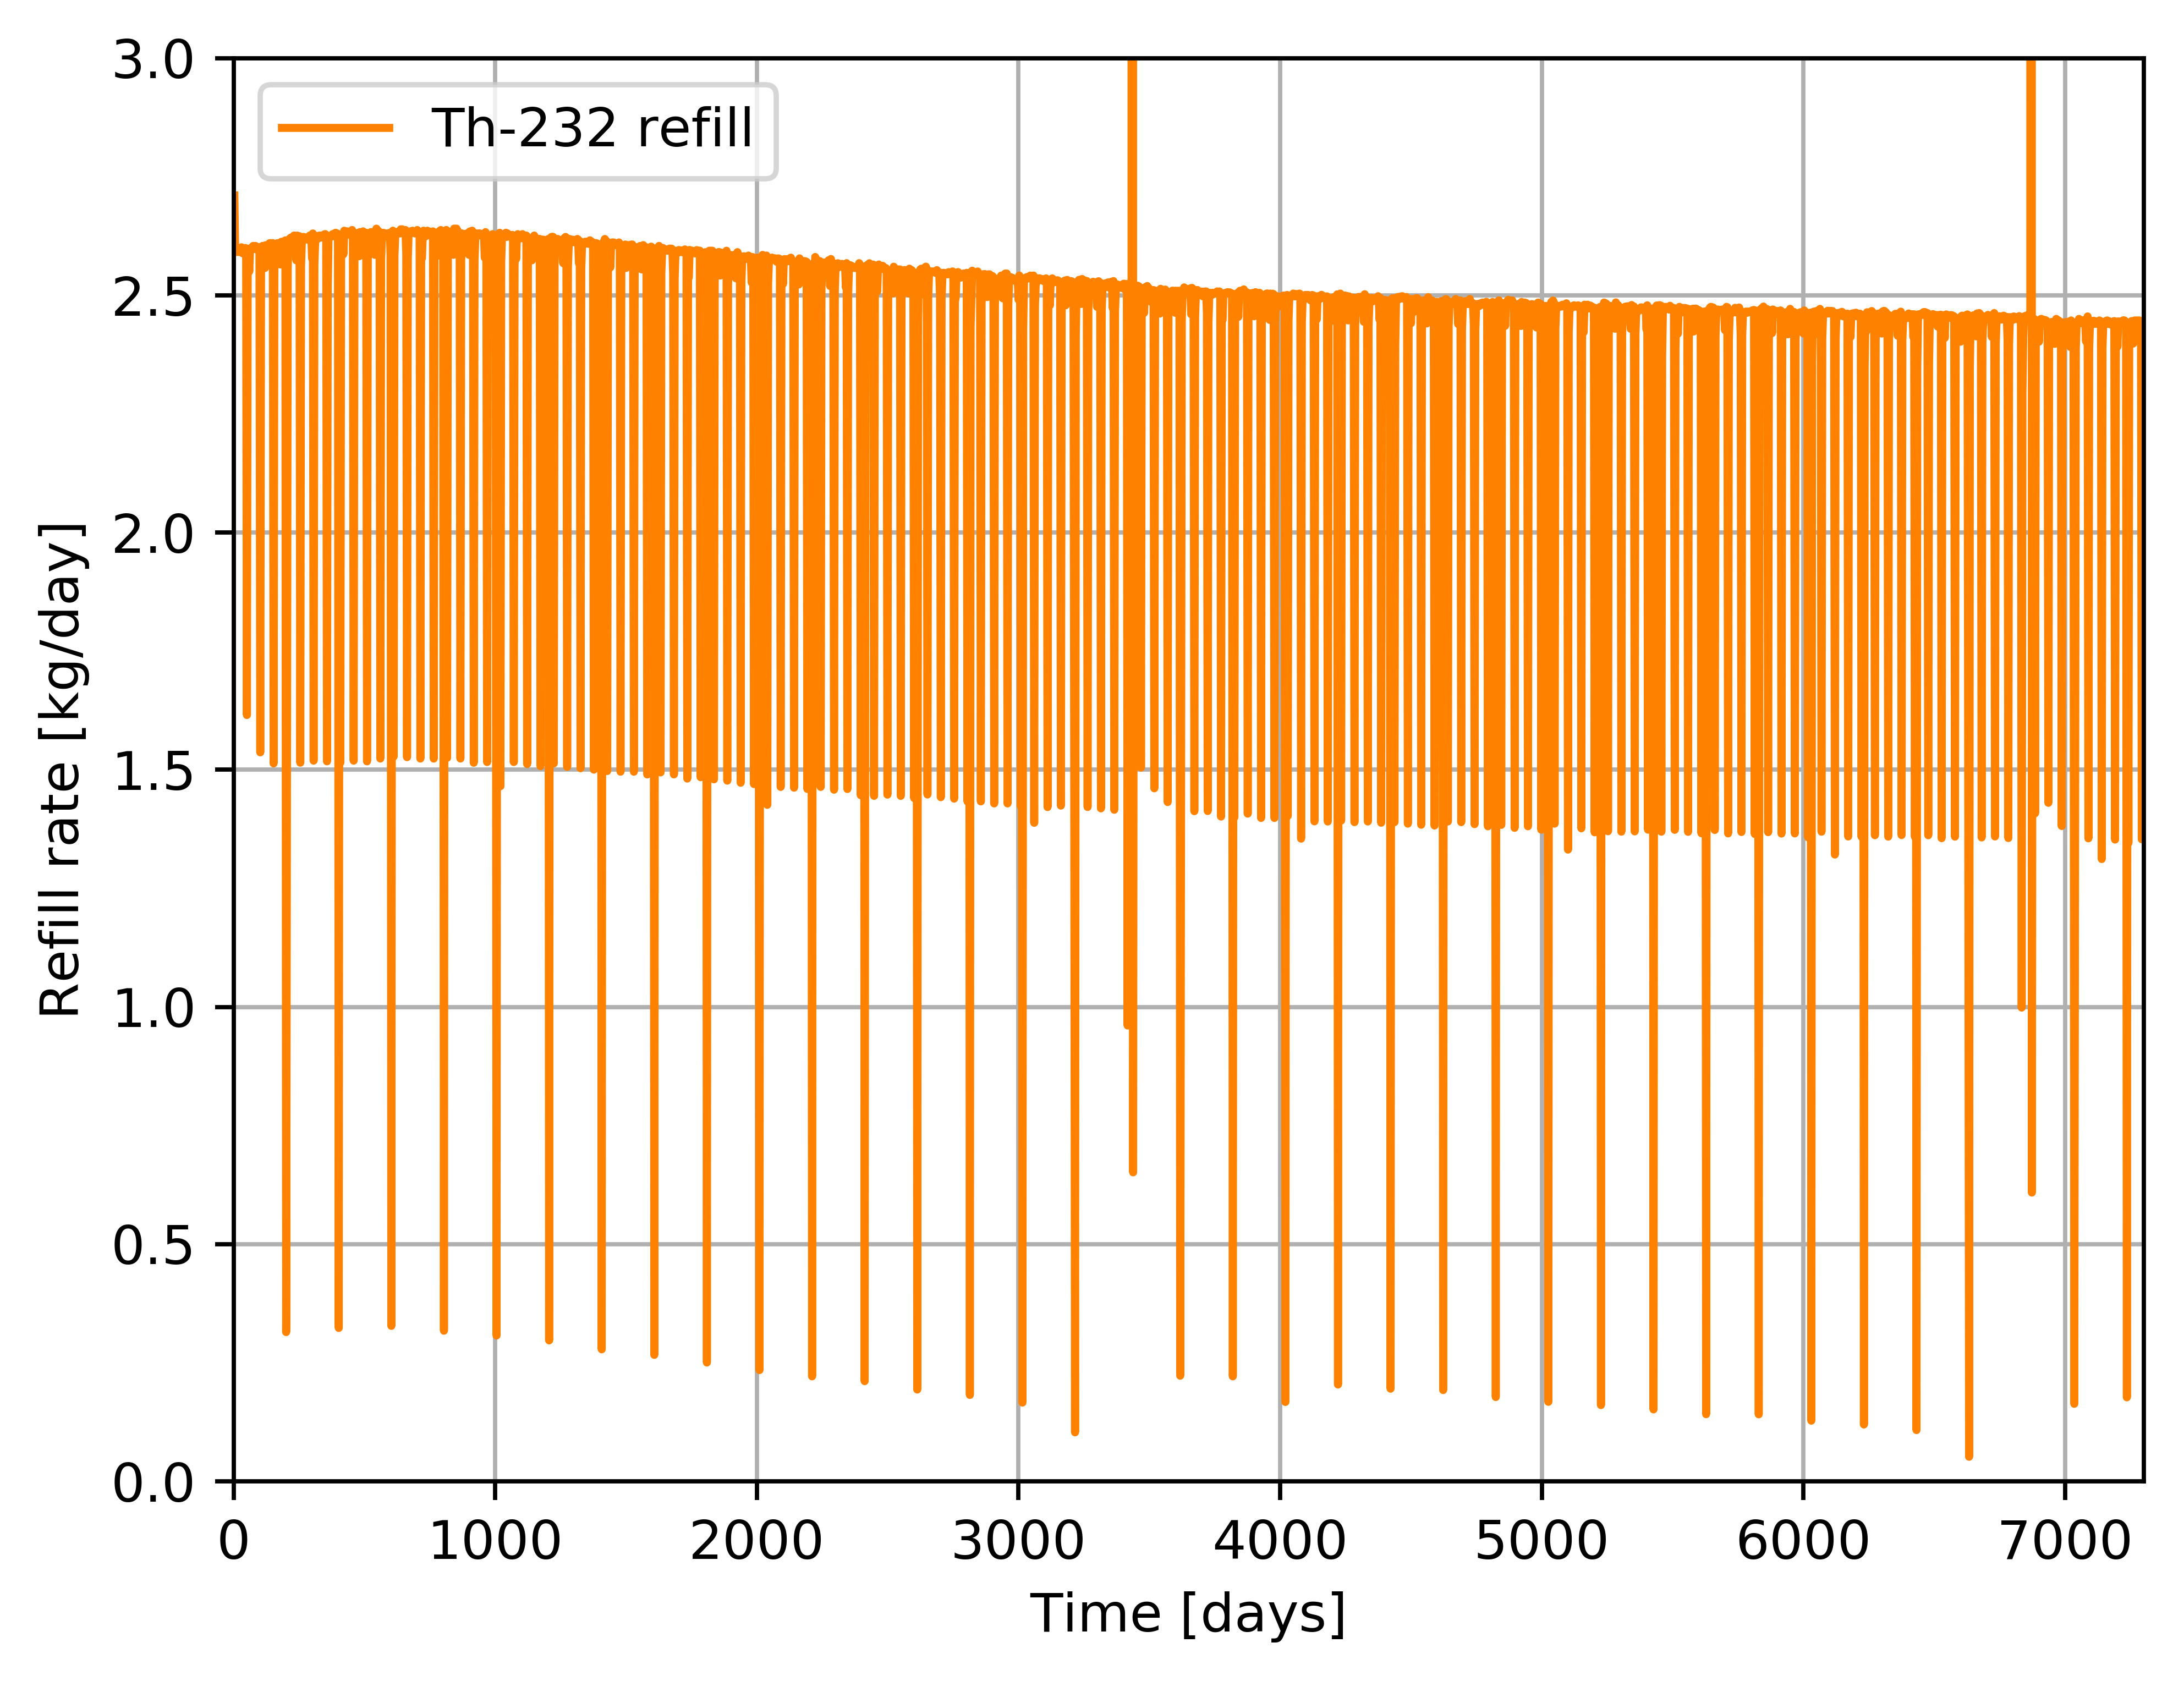
\includegraphics[width=\textwidth]{Th_refill_rate.png} \caption{$^{232}$Th 
  feed rate over 60 years of \gls{MSBR} operation.}
  \label{fig:th_refill}
\end{figure}

The average thorium feed rate increases during the first 500 days of operation, 
and steadily decreases due to spectrum hardening and accumulation of 
absorbers in the core. As a result, the average $^{232}$Th feed rate over 60 
years of operation is about 2.40 kg/day. This thorium consumption rate is in 
good agreement with a recent online reprocessing study by \gls{ORNL} 
\cite{betzler_molten_2017}. It must be noted that for the reactor with only 
thorium feed, at near equilibrium state, the thorium consumption rate is 
determined by the reactor power, the energy released per fission, and 
neutron energy spectrum.

\subsection{The effect of removing fission product from fuel salt}
Loading initial fuel salt composition into the \gls{MSBR} core leads to a 
supercritical configuration (Figure ~\ref{fig:fp_removal}). After reactor 
startup, the effective multiplication factor for the case with volatile gases 
and noble metals removal is approximately 7500 pcm  higher than for case with 
no fission products removal. This significant impact on the reactor core is
achieved due to immediate removal (20 sec cycle time) and high absorption cross 
section of Xe, Kr, Mo, and other noble metals removed. The effect of rare earth 
element removal is considerable a few months after startup and reached 
approximately 5500 pcm after 10 years of operation. The rare earth elements were 
removed at a slower rate (50-day cycle time). Moreover, 
Figure~\ref{fig:fp_removal} demonstrates that batch-wise removal of strong 
absorbers every 3 days did not necessarily leads to fluctuation in results 
but rare earth elements removal every 50 days causes an approximately 600 pcm jump 
in reactivity.

The effective multiplication factor of the core reduces gradually over 
operation time because the fissile material ($^{233}$U) continuously depletes 
from the fuel salt due to fission while fission products 
accumulate in the fuel salt simultaneously. Eventually, without fission products removal, 
the reactivity decreases to the subcritical state after approximately 500 and 
1300 days of operation for cases with no removal and volatile gases \& noble 
metals removal, respectively. The time when the simulated core reaches 
subcriticality ($k_{eff}<$1.0) for full-core model) is called the core lifetime. 
Therefore, removing fission products provides with significant neutronic benefit 
and enables a longer core lifetime.
\begin{figure}[ht!] % replace 't' with 'b' to force it to 
  \centering
  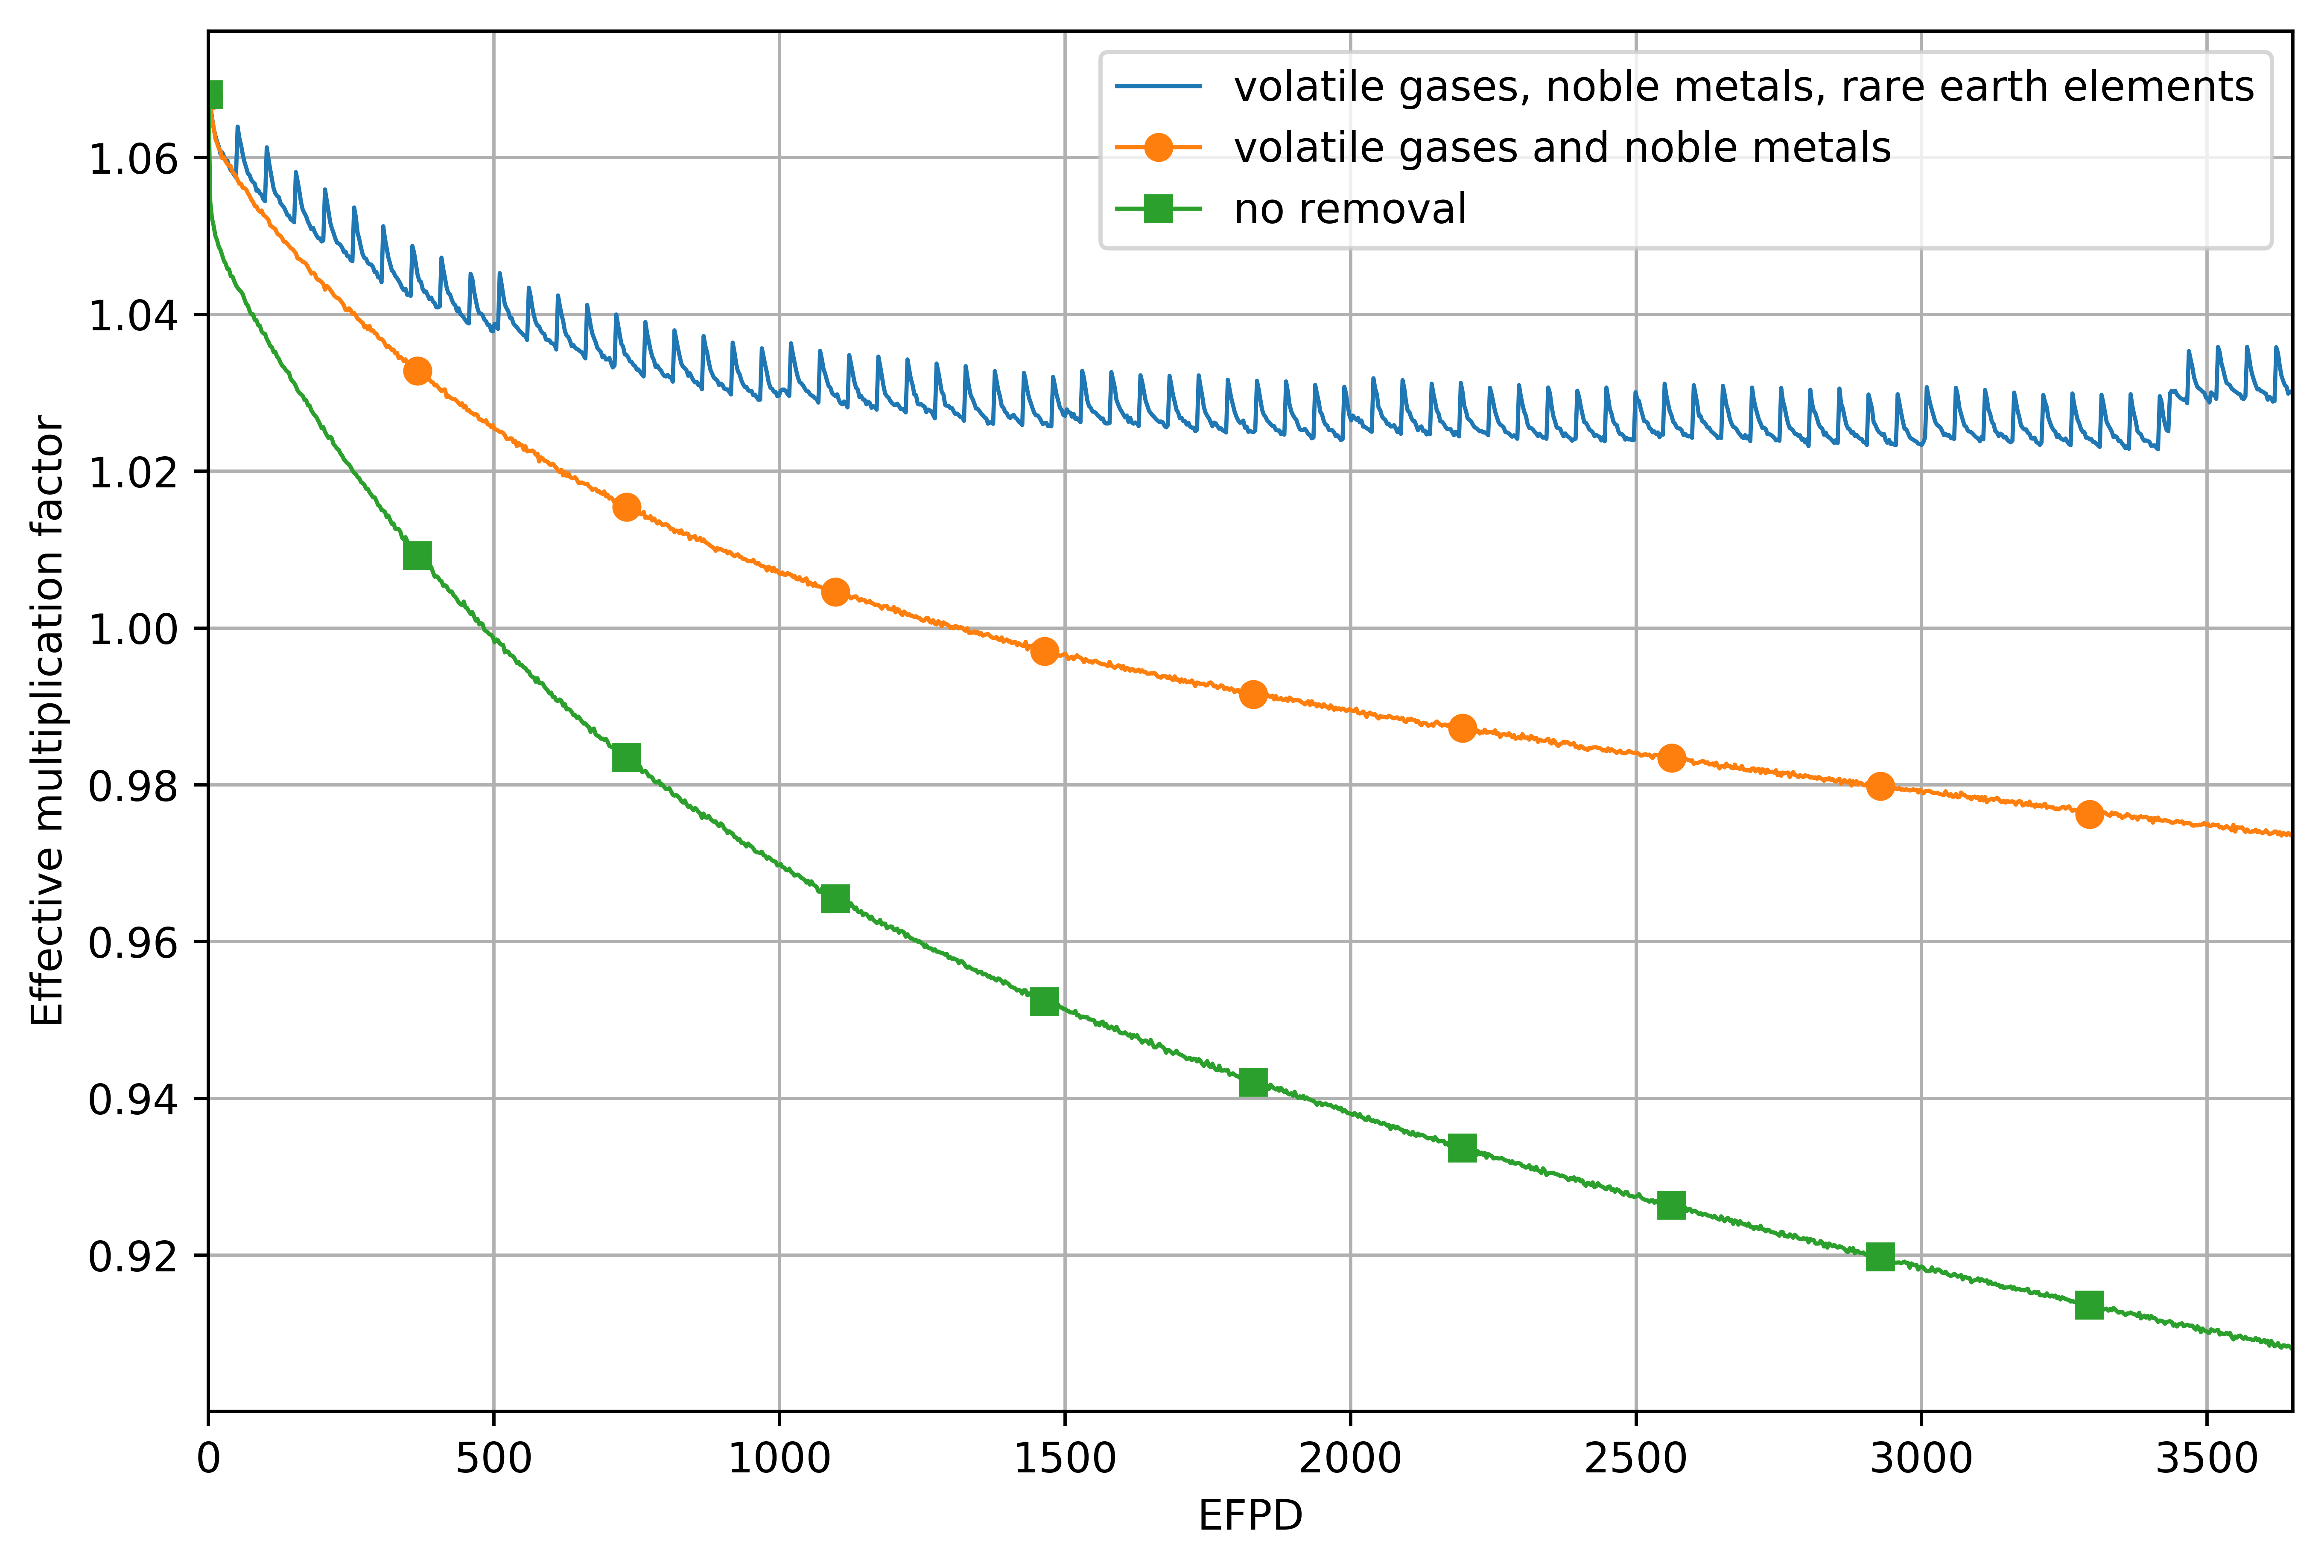
\includegraphics[width=\textwidth]{keff_rem_cases.png} 
  \caption{Calculated effective multiplication factor for full-core \gls{MSBR} 
model with removal of various fission product groups over 10 years of 
operation.}
  \label{fig:fp_removal}
\end{figure}
